\documentclass[final,12pt]{colt2018}

\usepackage[english]{babel}
\usepackage[utf8x]{inputenc}
%\usepackage{geometry}
%\usepackage{amsmath}
%\usepackage{amsfonts}
%\usepackage{soul}
%\usepackage{amssymb}
%\usepackage{graphicx}
%\usepackage{rotating}
%\usepackage{amsbsy}
%\usepackage{a4wide}
%\usepackage{graphicx,  ucs}
%\usepackage{float}
%\usepackage{tikz}
%\usepackage{algorithm}
%\usepackage[noend]{algpseudocode}
%\usepackage{listings}
\usepackage{enumitem}
%\usepackage{times}
\usepackage{hyperref}
%\usepackage{multirow}
%\usepackage{array}
%\usepackage[compact]{titlesec}
%% These have been added at the request of the MIT Libraries, because
%% some PDF conversions mess up the ligatures.  -LB, 1/22/2014
%\usepackage{cmap}
%\usepackage[T1]{fontenc}
\usepackage{bm}
\usepackage{comment}

\title[Certified Computation from Unreliable Datasets]{Certified Computation from Unreliable Datasets}
\usepackage{times}



% Compact itemize and enumerate.  Note that they use the same counters
% and symbols as the usual itemize and enumerate environments.
\def\compactify{\itemsep=0pt \topsep=0pt \partopsep=0pt \parsep=0pt}
\let\latexusecounter=\usecounter
%\newenvironment{CompactItemize}
%  {\def\usecounter{\compactify\latexusecounter}
%   \begin{itemize}}
%  {\end{itemize}\let\usecounter=\latexusecounter}
\newenvironment{CompactEnumerate}
  {\def\usecounter{\compactify\latexusecounter}
   \begin{enumerate}}
  {\end{enumerate}\let\usecounter=\latexusecounter}
\newenvironment{Itemize}%
{\begin{itemize}%
\setlength{\itemsep}{0pt}%
\setlength{\topsep}{0pt}%
\setlength{\partopsep}{0 in}%
\setlength{\parskip}{0 pt}}%
{\end{itemize}}

\newenvironment{pproof}
{ \noindent \textit{Proof.}  }
{ \hfill \rule{1.5ex}{1.5ex} }

\newcommand{\Domain}{\mathcal{D}}
\newcommand{\Support}{\mathcal{X}}
\newcommand{\Set}{S_{\mathcal{X}}}


% paper specific commands
\newcommand{\Workers}{\mathcal{N}}
\newcommand{\Truth}{\mathcal{T}}
\newcommand{\xw}{\vec{x}_{\Workers}}
\newcommand{\xt}{\vec{x}_{\Truth}}
\newcommand{\xs}{\vec{x}_{S}}

\newcommand{\Pow}{\mathrm{Pow}}
\newcommand{\PPow}{\mathrm{pPow}}
\newcommand{\Expo}{\mathrm{Exp}}
\newcommand{\Exp}{\mathbb{E}}
\newcommand{\tl}{\textlatin}
\newcommand{\tg}{\textgreek}
\newcommand{\RR}{\mathbb{R}}
\newcommand{\NN}{\mathbb{N}}
\newcommand{\pos}{\text{pos}}
\newcommand{\argmax}{\text{argmax}}
%\newcommand{\ver}{\text{VER}}
\newcommand{\argmin}{\text{argmin}}
\newcommand{\Neg}{\text{Neg}}
\newcommand{\appr}[1]{\(#1\)-\tl{approximation}}
\newcommand{\apprf}[2]{\(\frac{#1}{#2}\)-\tl{approximation}}
\newcommand{\com}[1]{}

%\newcommand{\ham}{\mathcal{H}}
%
%\definecolor{myC}{rgb}{0, 255, 255}
%\definecolor{myY}{rgb}{204, 204, 0}
%\definecolor{myM}{rgb}{255, 0, 255}
%
%

\def\poly{\mathrm{poly}}
\def\eps{\varepsilon}
\def\union{\cup}
\def\bigunion{\bigcup}
\def\cut{\cap}

\def\floor#1{\mathop{\left\lfloor#1\right\rfloor}}
\def\ceil#1{\mathop{\left\lceil#1\right\rceil}}
\def\Prob{\mathbb{P}}
\def\Exp{\mathbb{E}}
\def\Alg{\textsc{Alg}}
\def\Sub{\textsc{Sub}}
\def\Cond{\textsc{Cond}}
\def\EP{\textsc{EP}}
\def\SE{\textsc{SE}}
\def\DV{\textsc{DV}}
\def\MAX{\textsc{Max}}
\def\ARGMAX{\textsc{ArgMax}}
\def\SUM{\textsc{Sum}}
\def\WCOND{\textsc{WCond}}
\def\DES{\textsc{DES}}
\def\TIME{\textsc{TIME}}
\def\SPACE{\textsc{SPACE}}
\def\PSPACE{\textsc{PSPACE}}
\def\PLS{\textsc{PLS}}
\def\PPA{\textsc{PPA}}
\def\PPP{\textsc{PPP}}
\def\PPAD{\textsc{PPAD}}
\def\PPADS{\textsc{PPADS}}
\def\CLS{\textsc{CLS}}
\def\P{\textsc{P}}
\def\FP{\textsc{FP}}
\def\NP{\textsc{NP}}
\def\FNP{\textsc{FNP}}
\def\TFNP{\textsc{TFNP}}
\def\coNP{\textsc{coNP}}
\def\Banach{\textsc{NonMetricBanach}}
\def\Banachh{\textsc{Banach}}
\def\clocal{\textsc{Continuous LocalOpt}}

\newcommand{\reals}{\mathbb{R}}
\newcommand{\nats}{\mathbb{N}}

\def\OPT{\mathrm{OPT}}
\def\Int{\mathrm{Int}}
\def\Clos{\mathrm{Clos}}
\def\SC{\mathrm{SC}}
\def\MC{\mathrm{MC}}
\def\sw{\mathrm{sw}}
\def\mw{\mathrm{mw}}
\def\Ver{\mathrm{Ver}}
\def\ExpVer{\Exp\mathrm{Ver}}
\def\e{\epsilon}
\def\cost{\mathrm{cost}}

\def\norm#1{\left\|#1\right\|}
\def\normm#1{\left\|#1\right\|_{\Sigma}}
\def\abs#1{\left|#1\right|}
\def\matr#1{\mathbf{#1}}

\DeclareMathOperator*{\Min}{min}
\DeclareMathOperator*{\ver}{VER}
\newcommand{\correct}{\emph{correct}}
\newcommand{\wrong}{\emph{wrong}}
\renewcommand{\vec}{\mathbf}
\renewcommand{\l}{\vec{\lambda}}
\newcommand{\m}{\vec{\mu}}
\renewcommand{\v}{\vec{v}}
\newcommand{\diam}[2]{\mathrm{diam}_{#1}\left[ #2 \right]}

\definecolor{vergreen}{RGB}{0,85,2}
\definecolor{myvergreen}{RGB}{0,140,3}
\definecolor{provorange}{RGB}{85,34,0}
\definecolor{inputblue}{RGB}{5,13,111}
\definecolor{noapred}{RGB}{116,3,3}
\definecolor{classesblue}{RGB}{9,49,146}

\definecolor{secinhead}{RGB}{249,196,95}

\definecolor{lgray}{gray}{0.8}

 \coltauthor{\Name{Themis Gouleakis} \Email{tgoule@mit.edu}\\
 \addr EECS and CSAIL, MIT
 \AND
 \Name{Christos Tzamos} \Email{tzamos@mit.edu}\\
 \addr Microsoft Research
 \AND
 \Name{Manolis Zampetakis} \Email{mzampet@mit.edu}\\
 \addr EECS and CSAIL, MIT
 }

\begin{document}

\maketitle

\begin{abstract}
  A wide range of learning tasks require human input in labeling massive data.
  The collected data though are usually low quality and contain inaccuracies and
  errors. As a result, modern science and business face the problem of learning
  from unreliable data sets.

  In this work, we provide a generic approach that is based on
  \textit{verification} of only few records of the data set to guarantee high
  quality learning outcomes for various optimization objectives. Our method,
  identifies small sets of critical records and verifies their validity. We show
  that many problems only need $\poly(1/\eps)$ verifications, to ensure that the
  output of the computation is at most a factor of $(1 \pm \eps)$ away from the
  truth. For any given instance, we provide an \textit{instance optimal}
  solution that verifies the minimum possible number of records to approximately
  certify correctness. Then using this instance optimal formulation of the
  problem we prove our main result: ``every function that satisfies some
  Lipschitz continuity condition can be certified with a small number of
  verifications''. We show that the required Lipschitz continuity condition is
  satisfied even by some $\NP$-complete problems, which illustrates the
  generality and importance of this theorem.

  In case this certification step fails, an invalid record will be identified.
  Removing these records and repeating until success, guarantees that the result
  will be accurate and will depend only on the verified records. Surprisingly,
  as we show, for several computation tasks more efficient methods are possible.
  These methods always guarantee that the produced result is not affected by the
  invalid records, since any invalid record that affects the output will be
  detected and verified.
\end{abstract}

\begin{keywords}
  unreliable data set, verification, Lipschitz continuity
\end{keywords}

  % !TEX root = onlinevarinancebandits.tex

\section{Introduction}
% Structure:
% \begin{itemize}
% \item The approach of (Regularized) ERM and its importance in Machine Learning.
% Solving such problems with sequential optimization algorithms such as SGD/SVRG/Online K-means.
% Maybe focus on SGD as a running example.
% \item  Mentioned the alternative option is uniform sampling. Describe/illustrate how importance sampling can be used to improve the performance. Give references. 
% \item Describe how the variance of the estimates is a natural measure of performance in this setting. Mention that low variance translates to better performance, e.g. for SGD. 
% \textbf{Online Problem:}
% Similarly to  Duchi/EPFL  we formulate importance sampling an online convex optimization problem.
% Describe the approaches of Duchi/EPFL say very nice things about them give them credit and discuss the limitations of their results/approaches.
% \item State our result. State our contributions+ discuss the improvements over previous work: \\
% (i) tighter regret guarantees with respect to the simplex.\\
% (ii) Showing that regret minimization makes sense in this setting.\\
% (iii) (Hopefully) complementary lower bounds. \\
% (iii) Efficient experimental implementation showing the benefits of the proposed method
% \kl{This is for COLT, for ArXiv put the experiments in (ii) place}

% Discuss the technical challenges of our work, specifically the fact that the costs are unbounded + the bandit feedback.
% Discuss the new regularization that we introduce, its benefits (closed form formula for the FTRL) + the challenge.
% Mention other settings with unbounded losses, e.g. log loss in portfolio selection.
 
%  \textbf{Related work}
%  Who should we cite? Look at Jaggi/Duchi/EPFL for references.

% \kl{Mention (where?) that we can use our approach for coordinate descent.}

% \end{itemize}
%Among the most important paradigms in machine learning is Empirical Risk Minimization (ERM) , which is often the strategy of choice due to its generality and statistical efficiency.
Empirical risk minimization (ERM) is among the most important paradigms in machine learning, and  is often the strategy of choice due to its generality and statistical efficiency.
In ERM, we draw a set of  samples $\D=\{x_1,\ldots,x_n\}\subset \X$ from the underlying data distribution, and we aim to find a solution $w\in\W$ that minimizes the empirical risk,  %The empirical risk serves as a proxy to the expected loss which is often. 
%the objective is to  find a solution $w\in\W$ that minimizes the empirical risk based on a collection of $n$ samples $\D=\{x_1,\ldots,x_n\}\subset \X $:
\begin{equation} \label{eq:ERM}
  \min_{w\in\W }L(w) := \frac{1}{n}  \sum_{i=1}^n \ell (x_i, w),
\end{equation}
where $\ell: \mathcal{X} \times \W \rightarrow \reals$ is a given loss function, and $\W\subseteq \reals^d$ is usually a compact domain.

In this work we are interested in sequential procedures for minimizing the ERM objective, and relate to such methods as \emph{ERM solvers}.
More concretely, we focus on the regime where the number of samples $n$ is very large,  and it is therefore desirable to employ ERM solvers that only require  few passes over the dataset. There exists a rich arsenal of such efficient solvers which have been investigated throughout the years, with the canonical example from this category being  Stochastic Gradient Descent (SGD).


% among are SVRG \citep{johnson2013accelerating} and SAGA \citep{defazio2014saga},
%
%
% such efficient sequential solvers have been developed throughout the years, with the canonical example from this category being  Stochastic Gradient Descent (SGD).

Typically, such methods  require an unbiased estimate of the loss function at each round, which is usually  generated   by sampling a few points uniformly at random from the dataset.
However, by employing uniform sampling, these methods are insensitive to the intrinsic structure of the data. In case of SGD, for example, some data points might produce large gradients, but they are nevertheless assigned the same probability of being sampled as any other point. This ignorance often results in high-variance estimates, which is likely to degrade the performance.

The above issue can be mended by employing non-uniform importance sampling.
And indeed, we have recently witnessed several  techniques to do so: %techniques.
%In recent years several approaches have been developed in order to address this issue.
\citet{zhao2015stochastic} and similarly \citet{needell2014stochastic}, suggest using prior knowledge on the gradients of each data point in order to devise predefined importance sampling distributions.  \citet{NIPS2017_7025} devise adaptive sampling techniques guided by a robust optimization approach. These are only a few examples of a larger body of work 
 \citep{bouchard2015online, alain2015variance, csiba2016importance}.

Interestingly, the recent works of \cite{pmlr-v70-namkoong17a} and \cite{salehi2017} formulate the task of devising importance sampling distributions as an online learning problem with bandit feedback. In this context, they  think of the algorithm, which adaptively chooses the distribution, as a player that competes against the ERM solver. The goal of the player is to minimize the cumulative variance of the resulting (gradient) estimates.  Curiously, both methods rely on some form of the ``linearization trick''\footnote{ By ``linearization trick'' we mean that these methods update according to a first order approximation  of the costs rather than the costs themselves.} 
%\footnote{If $g_t$ is a subgradient of the convex function $f:S\rightarrow \mathbb{R}$ at $w_t$, then $f(w_t) - f(u) \leq (w_t-u)^\intercal g_t$,  $\forall u \in S$.} 
 to resort to the analysis of the EXP3  \citep{auer2002nonstochastic}.

On the other hand, the theoretical guarantees of the above methods are somewhat limited. Strictly speaking, none of them provides regret guarantees with respect to the best fixed distribution in hindsight:  \citet{pmlr-v70-namkoong17a} only compete with the best distribution among a \emph{subset} of the simplex (around the uniform distribution).  Conversely, \cite{salehi2017} compete against a solution which might perform worse than the best in hindsight up to a multiplicative factor of $3$.

In this work, we adopt the above mentioned online learning formulation, and design novel importance sampling techniques. 
Our adaptive sampling procedure is simple and efficient, and 
in contrast to previous work, we are able to provide regret guarantees with respect to the best fixed point among the simplex.
As our contribution, we
\vspace{-1.5mm}
\begin{itemize}
\setlength\itemsep{0.05em}
\item motivate theoretically why regret minimization is meaningful in this setting, 
\item propose a novel bandit algorithm for variance reduction ensuring regret  of~$\tO(n^{1/3}T^{2/3})$,
\item empirically validate our method, and provide an efficient implementation\footnote{The source code is available at  \url{https://github.com/zalanborsos/online-variance-reduction}}.
\end{itemize}
On the technical side, we do not rely on a ``linearization trick'' but rather directly employ a scheme based on the classical 
 Follow-the-Regularized-Leader approach. 
Our analysis entails several technical challenges, most notably handling  unbounded cost functions while only receiving partial (bandit) feedback. Our design and analysis draws inspiration from the seminal works of  \citet{auer2002nonstochastic}  and 
\cite{Abernethy08}. 
Although we present our method for choosing \emph{data points}, it naturally applies to choosing \emph{coordinates in coordinate descent} or even \emph{blocks} of thereof \citep{allen2016even,perekrestenko2017faster, nesterov2012efficiency, necoara2011random}.
More broadly, the proposed algorithm can be incorporated in \emph{any sequential algorithm} that relies on an unbiased estimation of the loss. A prominent  application of our method is variance reduction for SGD, which can be achieved by considering  gradient norms as  losses, i.e., replacing $\ell(w,x_i) \leftrightarrow \|\nabla \ell(w,x_i)\|$. With this modification, our method is minimizing the cumulative variance of the gradients throughout the optimization process.

%defining the bandit feedback as the norm of the gradient estimate. 
The paper is organized as follows. In Section \ref{sec:Motivation}, we formalize the online learning setup of variance reduction, and motivate why regret is a suitable performance measure. As the first step of our analysis, we investigate the full information setting in Section \ref{sec:full-info}, which serves as a mean for studying the bandit setting in Section \ref{sec:bandit}. Finally, we validate our method empirically, and provide the detailed discussion of the results in Appendix  \ref{sec:experiments}. 



%We achieve this by relying on classical results from Follow-the-Regularized-Leader framework, where the regularizer is chosen to suit the setting of variance reduction with importance sampling.

%\newpage
%
%
% rely on solving a a ro
%
%There exists
%
%In 
%Addressing the regime where the number of samples $n$ is very large, efficient \emph{sequential} procedures have been developed, that perform only a few passes over the dataset. These methods usually require an unbiased estimate of the loss function at each round, and they generate the estimate by sampling a few points uniformly at random from the dataset. The canonical example from this category is Stochastic Gradient Descent (SGD).
%
%However, by employing uniform sampling, these methods are agnostic to the intrinsic structure of the data. In case of SGD, for example, some data points might produce large gradients, but they are nevertheless assigned the same probability of being sampled as any other point. This ignorance often results in high-variance estimates.
%
%References:
%\begin{itemize}
%\item \textbf{Variance reduction with uniform sampling}: SVRG \citep{johnson2013accelerating} and SAGA \citep{defazio2014saga}, \cite{xiao2014proximal}
%\item \textbf{Variance reduction with importance sampling (points): } \citep{needell2014stochastic, zhao2015stochastic, bouchard2015online, csiba2016importance,alain2015variance, NIPS2017_7025}
%\item \textbf{Importance sampling, but without direct interpretation as variance reduction (points): } \cite{strohmer2009randomized}, 
%\item \textbf{Coordinate descent, with non-uniform sampling:} \cite{allen2016even,perekrestenko2017faster, nesterov2012efficiency, necoara2011random}
%\item \textbf{Bandits, both points and coordinates:} \cite{pmlr-v70-namkoong17a}, \cite{salehi2017}, \cite{salehi2017stochastic}
%\end{itemize}
%
%
%This issue is addressed by several variance reduction techniques, some prominent examples being  SVRG \citep{johnson2013accelerating} and SAGA \citep{defazio2014saga}. In case of (strongly) convex loss functions, the reduced variance directly translates to improved convergence bounds. \textcolor{red}{An important class of methods that allow variance reduction interpretation}  rely on the technique of importance sampling \citep{needell2014stochastic, zhao2015stochastic, bouchard2015online, csiba2016importance,alain2015variance%, allen2016even, perekrestenko2017faster%
%, NIPS2017_7025}, where the sampling distribution is either fixed or adaptive over the iterations. Since competing against \textcolor{red}{the optimal per-round} sampling distributions is usually computationally infeasible, the methods are often compared to the optimal sampling distribution \emph{in hindsight}.
%
%An interesting idea of the recent works of \cite{pmlr-v70-namkoong17a} and \cite{salehi2017} is to formulate the task of finding a competitive sampling distribution under importance sampling for variance reduction as a \emph{bandit problem}. In this setting, no-regret assures that the chosen distribution performs close to the optimal stationary distribution in hindsight. Both methods rely on some form of the ``linearization trick'' \citep{shalev2012online} to resort to the analysis of the EXP3  \citep{auer2002nonstochastic} and obtain similar algorithms. These methods show convincing convergence guarantees for stochastic optimization for convex ERM both theoretically and empirically.
%
%On the other hand, the two methods come with limitations. While the latter is guaranteed to approximate the variance under the optimal sampling distribution in hindsight within a factor of 3, the former incorporates a KL-projection step in order to ensure that the sampling probabilities are larger than some threshold $\pmin$ --- an additional hyperparameter that affects the convergence bounds.
%
%In this work, we pursue the same idea of employing bandit optimization for variance reduction and we design an algorithm that suffers from none of the limitations mentioned above. We achieve this by relying on classical results from Follow-the-Regularized-Leader framework, where the regularizer is chosen to suit the setting of variance reduction with importance sampling. As our contribution, we
%\vspace{-1.5mm}
%\begin{itemize}
%\setlength\itemsep{0.05em}
%\item motivate theoretically why regret minimization is meaningful in this setting,
%\item propose and analyze a novel bandit algorithm for variance reduction,
%\item empirically validate our method and provide an efficient implementation\footnote{The source code is available at  \url{https://github.com/zalanborsos/online-variance-reduction}}.
%\kl{Dont forget to remove this footnote in the anonimized COLT submission!}
%\end{itemize}
%The analysis entails several technical challenges, most notably handling  unbounded cost functions and unbounded regularizers. Although we present our method for choosing \emph{datapoints} in an optimization problem, it naturally applies to choosing \emph{coordinates in coordinate descent} or even \emph{blocks} of thereof. More broadly, the proposed algorithm can be incorporated in \emph{any sequential algorithm} that relies on unbiased estimation of the loss.
%\kl{add citation about coordinate descent, see Cevher and Jaggi}

  \section{Property Testing Background and Models}
\label{sec:model}
\subsection{Query Testing (Standard Property Testing)}
Given functions $f$ and $g$ over domain $X$, we define the distance between $f$ and $g$ with respect to distribution $\calD$ over $X$ to be
\begin{equation}
\dist_\calD(f,g)=\Pr_{x\sim\calD}[f(x)\neq g(x)].
\end{equation}
Given a class $\calC$ of functions over domain $X$ and a margin $\epsilon$, a \emph{property tester} distinguishes the case that the input function $f$ is in the class $\calC$ from the case that $f$ is $\epsilon$-far from $\calC$:
\begin{enumerate}
\item if $f\in\calC$, the tester accepts $f$ with probability at least $\frac{2}{3}$;
\item if $\forall g\in\calC,\dist_\calD(f,g)>\epsilon$, the tester rejects $f$ with probability at least $\frac{2}{3}$.
\end{enumerate}
\citet{RS96} first studied the property testing model assuming $X$ is finite and $\calD$ is uniform. We call the testing model of \citet{RS96} as \emph{query testing}, because the tester makes queries to access $f$, i.e., the tester asks for the value of $f(x)$ for some $x\in X$ for each query it makes.

\citet{PRR06} first studied the \emph{tolerant} version of property testing: given an additional parameter, the threshold $\alpha$, to distinguish a function $\alpha$-close to the class from a function $(\alpha+\epsilon)$-far from the class. In other words, 
\begin{enumerate}
\item if $\exists g\in \calC,\dist_\calD(f,g)\leq\alpha$, the tester accepts $f$ with probability at least $\frac{2}{3}$;
\item if $\forall g\in\calC,\dist_\calD(f,g)>\alpha+\epsilon$, the tester rejects $f$ with probability at least $\frac{2}{3}$.
\end{enumerate}
They showed tolerant testers for clustering and for monotonicity in the query testing model. \citet{FF05} showed the existence of classes of binary functions that are efficiently query-testable in the non-tolerant case but are not efficiently query-testable in the tolerant case.

\citet{PRR06} also considered a similar task called distance approximation: estimating the distance from the function to the class so that with probability at least $\frac 23$ the output is within $\pm\epsilon$ to the true distance. Note that distance approximation with additive error $\epsilon$ implies tolerant testing with margin $2\epsilon$ with the same query complexity. Based on this observation, all the tolerant testers we design in this paper actually perform distance approximation (so we don't need the parameter $\alpha$) because distance approximation is a slightly more convenient model for our presentation.
\subsection{Passive Testing (Sample-Based Testing)}
\label{subsec:passive}
\citet{GGR98} first studied testers with the ability to obtain a random sample in addition to making queries so that the tester can potentially work on arbitrary distributions (see Section \ref{subsec:distributionfree} for distribution-free testing), although their algorithmic results remained in the query testing framework over the uniform distribution.
\citet{KR98} developed the first \emph{passive} testers, testers that don't make queries and only rely on the random i.i.d.\ sample to access the input function $f$, for a variety of classes with sub-learning sample complexity. \citet{GR13} advanced the study of passive testers by providing several general positive results as well as by revealing relations with other testing models.

\emph{Proper} learning implies testing, simply by testing using the output hypothesis, but passive testing can be substantially harder than \emph{improper} learning. \citet{GGR98} pointed out that the class of $k$-term-DNF is NP-hard for non-tolerant passive testing while it is efficiently PAC learnable via $k$-CNF \citep{PV88}, if we require testing and learning on an arbitrary distribution.

The general hardness of \emph{tolerant} passive testing based on hardness of improper \emph{agnostic} learning can be implied from the recent work by \citet{KL18}. They considered the task of refutation: for any fixed distribution $\calD$ over domain $X$, given a sample of example-label pairs $\{(x_i,y_i)\}$ and margin $\epsilon>0$, to distinguish the following two cases:
\begin{enumerate}
\item accept when every $(x_i,y_i)$ is i.i.d.\ from some distribution $\calD'$ over $X\times\{0,1\}$ with marginal on $X$ being $\calD$ and $\exists f\in\calC,\Pr_{(x,y)\sim\calD'}[f(x)\neq y]\leq\frac 12-\epsilon$;
\item reject when every $x_i$ is i.i.d.\ from $\calD$ and every $y_i$ is i.i.d.\ from the uniform distribution over $\{0,1\}$.
\end{enumerate}
They showed that a refutation algorithm for distribution $\calD$ with margin $\epsilon$ and sample complexity $s$ implies an improper agnostic learning algorithm for the same distribution with error $3\epsilon$ and sample complexity $O(\frac{s^3}{\epsilon^2})$. We show in Appendix \ref{sec:refutation} that the refutation algorithm can be reduced to a tolerant passive tester for arbitrary unknown distributions with threshold $\alpha=\frac 12-\frac{3\epsilon}4$, margin $\frac{\epsilon}{2}$, and sample complexity $\Omega(s)$, implying that tolerant passive testing for arbitrary unknown distributions can't be substantially more sample-efficient than improper agnostic learning for any distribution $\calD$ (with some reasonable assumptions about the distribution $\calD$). %The reduction also has a uniform-distribution version (Lemma \ref{}), implying the hardness of tolerant passive testing over the uniform distribution.

%\citet{Vad17} showed that if one can perform refutation, i.e., distinguishing a function in the class from a random function, using a sample of size $s$, then one can also do improper PAC learning with sample complexity $O(\poly(s))$.  \citet{KL18} showed similar results for the tolerant (agnostic) case. They used a different definition of refutation: distinguishing a function having distance $\frac 12-\epsilon$ to the class from a random function, and showed that if one can perform refutation using a sample of size $s(\epsilon)$, then one can also do improper agnostic learning with sample complexity $O(\frac{\left(s(\frac\epsilon 2)\right)^3}{\epsilon^2})$.\footnote{One difference between the two results is that \citet{Vad17} assumes that the distribution is arbitrary while the result by \citet{KL18} is distribution-specific. } Note that passive testing implies refutation with the same sample complexity both in the non-tolerant and the tolerant case, assuming the concept class has a finite VC-dimension and the distribution has no massive points so that a random function has distance $\frac 12$ to it with probability 1. Therefore these results imply that passive testing can't be substantially more sample-efficient than improper learning.

\subsection{Active Testing}
Both query testing and passive testing have shortcomings. The assumption of query testing that the tester can make queries to arbitrary points in the domain is usually impractical, while passive testing is too restrictive: for the tolerant case, passive testing can't be substantially more sample-efficient than agnostic learning (recall Section \ref{subsec:passive}).

To avoid both shortcomings, \citet{BBBY12} proposed the active testing model where the tester first receives an unlabeled random i.i.d.\ sample and then makes queries to points in the sample. While the size of the unlabeled sample might be comparable to the labeled sample complexity for learning, the number of queries the tester makes should be substantially smaller.
%large (but is still required to be polynomial in the VC-dimension of the class), the number of queries the tester makes should be substantially smaller than the sample complexity for learning. 
They showed (non-tolerant) active testers for unions of $d$ intervals and for linear separators.
\subsection{Distribution-Free Testing}
\label{subsec:distributionfree}
Distribution-free testing \citep{GGR98} considers testers that work on arbitrary unknown distributions with the ability to obtain random i.i.d.\ sample in addition to making queries. \citet{HK03} designed distribution-free testers for low-degree multivariate polynomials, monotone functions, and several other classes.

The difference between distribution-free testing and passive testing (over arbitrary unknown distributions) is that distribution-free testers have the ability to make queries while passive testers don't. However, the query ability is helpful only when we do \emph{non-tolerant} testing where the tester is only required to accept functions in the class, rather than functions having distance 0 to the class with respect to the unknown distribution. For \emph{tolerantly} testing binary functions, we show that distribution-free testing implies passive testing with the same sample complexity (see Section \ref{sec:relationship} Lemmas \ref{lm:distributionfreenontolerant} and \ref{lm:distributionfreetolerant}) and thus the hardness for tolerant passive testing extends automatically to tolerant distribution-free testing.



%\subsection{Property Testing, Tolerant Testing and Distance Approximation}
%Suppose we have a ground set $X$ and a distribution $\calD$ over $X$. For any two binary functions $f,g\in\{0,1\}^X$, we define their distance to be $\dist_{\calD}(f,g)=\Pr_{x\sim \calD}[f(x)\neq g(x)]$. 

%Suppose we also have a concept class $\calC\subseteq\{0,1\}^X$. Given a function $f\in\{0,1\}^X$ and a margin $\epsilon$ as input, the task of property testing $\pt_{\calD}(f,\epsilon)$ \citep{RS96} is to distinguish the case that $f$ belongs to class $\calC$ from the case that $f$ is $\epsilon$-far from $\calC$. In other words, $\forall f$,
%\begin{enumerate}
%\item if $f\in\calC$, the algorithm outputs ``YES'' with probability at least $\frac{2}{3}$;
%\item if $\forall g\in\calC,\dist_{\calD}(f,g)>\epsilon$, the algorithm outputs ``NO'' with probability at least $\frac{2}{3}$.
%\end{enumerate}
%A property testing algorithm may be randomized, and in this case, the goal is to output the correct answer with probability at least $\frac{2}{3}$. The success probability can be boosted to $1-\delta$ by repeating the algorithm for $O(\log\frac{1}{\delta})$ times and taking the majority.

%The function $f$ can be given to the algorithm in many different ways. In the \emph{query testing} framework \citep{RS96}, the algorithm can query the value of $f(x)$ for any $x\in X$. In this framework, we say the algorithm has \emph{query access} to $f$, or has access to $f\qu$. The query complexity of the algorithm, as a function of $\frac{1}{\epsilon}$, is measured by the maximum number of queries needed by the algorithm.

%\citet{BBBY12} argued that the query testing framework is not realistic for machine learning practice. They proposed the \emph{active testing} framework, in which the algorithm first requests $N$ unlabeled examples $x_1,x_2,\cdots,x_{N}\in X$ sampled independently according to $\calD$ and can only choose to query $f(x_i)$ for $1\leq i\leq N$. In this framework, we say the algorithm has \emph{active access} to $f$, or has access to $f\ac$. The maximum value of $N$, as a function of $\frac{1}{\epsilon}$, is called the \emph{unlabeled sample complexity}. The query complexity is still defined as a function of $\frac{1}{\epsilon}$ measuring the maximum number of queries needed by the algorithm.

%\citet{GGR98} and \citet{KR98} studied an even more strict way of accessing $f$, called \emph{passive access}, in which the algorithm is given the label of an example chosen independently at random from $\calD$ for each query the algorithm makes. 

%Tolerant testing $\tot_{\calD}(f,\alpha,\epsilon)$ \citep{PRR06} is a similar task to property testing. The only difference is that besides the margin $\epsilon$, we are given another parameter $\alpha$ as input, and we are asked to distinguish the case that $f$ is $\alpha$-close to $\calC$ from the case that $f$ is $(\alpha+\epsilon)$-far from $\calC$. %following two cases:
%\begin{enumerate}
%\item $\exists g\in\calC,\dist_{\calD}(f,g)\leq \alpha$;
%\item $\forall g\in\calC,\dist_{\calD}(f,g)>\alpha+\epsilon$.
%\end{enumerate} 
%The query complexity of tolerant testing is still measured as a function of $\frac{1}{\epsilon}$ \citep{PRR06}. 

%A natural generalization of tolerant testing is distance approximation, in which we are only given the function $f$ and the margin $\epsilon$ as input and required to output $\hat\alpha$ as an approximation of the distance from $f$ to $\calC$ up to an additive error $\epsilon$. More specifically, the goal of $\da_{\calD}(f,\epsilon)$ is to output $\hat\alpha$ such that $\forall f$,
%\begin{enumerate}
%\item $\forall \alpha$ such that $\exists g\in\calC,\dist_{\calD}(f,g)\leq \alpha$, it holds with probability at least $\frac{2}{3}$ that $\hat\alpha\leq \alpha+\epsilon$;
%\item $\forall \alpha$ such that $\forall g\in\calC,\dist_{\calD}(f,g)>\alpha$, it holds with probability at least $\frac{2}{3}$ that $\hat\alpha> \alpha-\epsilon$.
%\end{enumerate}

%The success probability of a distance approximation algorithm can be boosted to $1-\delta$ by repeating it $O(\log\frac{1}{\delta})$ times and taking the median. 

%Because for any $\calD$ and $\epsilon$, it's clear that a $\da_{\calD}(f,\frac{\epsilon}{2})$ algorithm implies a $\tot_{\calD}(f,\alpha,\epsilon)$ algorithm with the same query and unlabeled sample complexity \citep{PRR06}, we focus on distance approximation rather than tolerant testing throughout the paper.

%For all of the above examples, the distribution $\calD$ appears in the subscript meaning that the distribution is fixed and known to the algorithm. In this paper, we will consider a more general case, for example $\pt(f\qu,\epsilon,\calD)$, in which the distribution $\calD$ is arbitrarily given to the algorithm as input. When the algorithm has active or passive access to $f$, it's possible to consider an even more general case, for example $\pt(f\ac,\epsilon)$, in which the distribution $\calD$ is unknown to the algorithm (but implicitly given to the algorithm when accessing $f$).




%We use $q^{\text{query}}(\epsilon)$ and $q^{\text{active}}(\epsilon)$ to denote the maximum number of queries needed in the query testing model and the active testing model, respectively. \citet{BBBY12} showed that $q^{\text{query}}(\epsilon)\leq q^{\text{active}}(\epsilon)$ always holds for non-tolerant property testing, which can be easily generalized to tolerant testing and distance approximation. They also showed for non-tolerant property testing that when $\calC$ is the class of dictator functions and $\calD$ is the uniform distribution over $\{0,1\}^p$, there is a testing algorithm in the query testing framework whose query complexity $q^{\text{query}}(p,\epsilon)$ does not grow with respect to $p$, while every testing algorithm in the active testing framework requires $q^{\text{active}}(p,\epsilon)=\Omega(\log p)$ queries for any fixed $0<\epsilon<\frac{1}{2}$.

%In this paper, however, we will show in Theorem \ref{thm:unlabeled} a reversed inequality that $q^{\text{active}}(\epsilon)=O(q^{\text{query}}(\frac{\epsilon}{2}))$ when we are required to do testing on \emph{arbitrary} distribution $\calD$ and the queries are required to lie in the support of $\calD$ (when we have query access)\footnote{We can assume without loss of generality that the queries all lie in the support of $\calD$ when we do tolerant testing and distance approximation, but we cannot assume this for non-tolerant property testing. The reason is that $f\in\calC$ is stronger than $\exists g\in\calC,\dist_{\calD}(f,g)=0$.}, uncovering the relationship between query access and active access.


%Similar to Theorem \ref{thm:unlabeled}, we have the following theorem in tolerant testing. Its proof is a simple modification of the proof to Theorem \ref{thm:unlabeled}.






  % !TeX root = main.tex
\section{Certification Schemes for Linear Programs} \label{sec:certification}

  In this section, we present examples of certification schemes for frequently arising problems such as computing the sum 
of values or functions that can be expressed as a linear programs. In the next section we will see the more general statement
about certification schemes for functions that satisfy a general Lipschitz continuity condition.

\subsection{Computing the Sum of Records} \label{ssec:certificationSum}

  One of the most basic certification tasks is computing the sum of the values of the records. For this task, we are given $n$ 
positive real numbers $x_1, x_2, \dots, x_n$ each one comming from a record in our data set. Our goal is to certify whether the
sum of all the records is closed to the sum of the subset of records that are valid, i.e. belong to $\Truth$. 

  More formally, we want to check with probability of failure at most $\delta > 0$ whether 
$\sum_{i \in \Workers} x_i \in \left[1 - \eps, \frac{1}{1 - \eps} \right] \cdot \sum_{i \in \Truth} x_i$ or there is at least 
one record $i$ such that $i \notin {\cal T}$. We show that there exists an efficient certification scheme for this task:

\begin{figure}[!h] \label{fig:certification sum}
  \centering
  {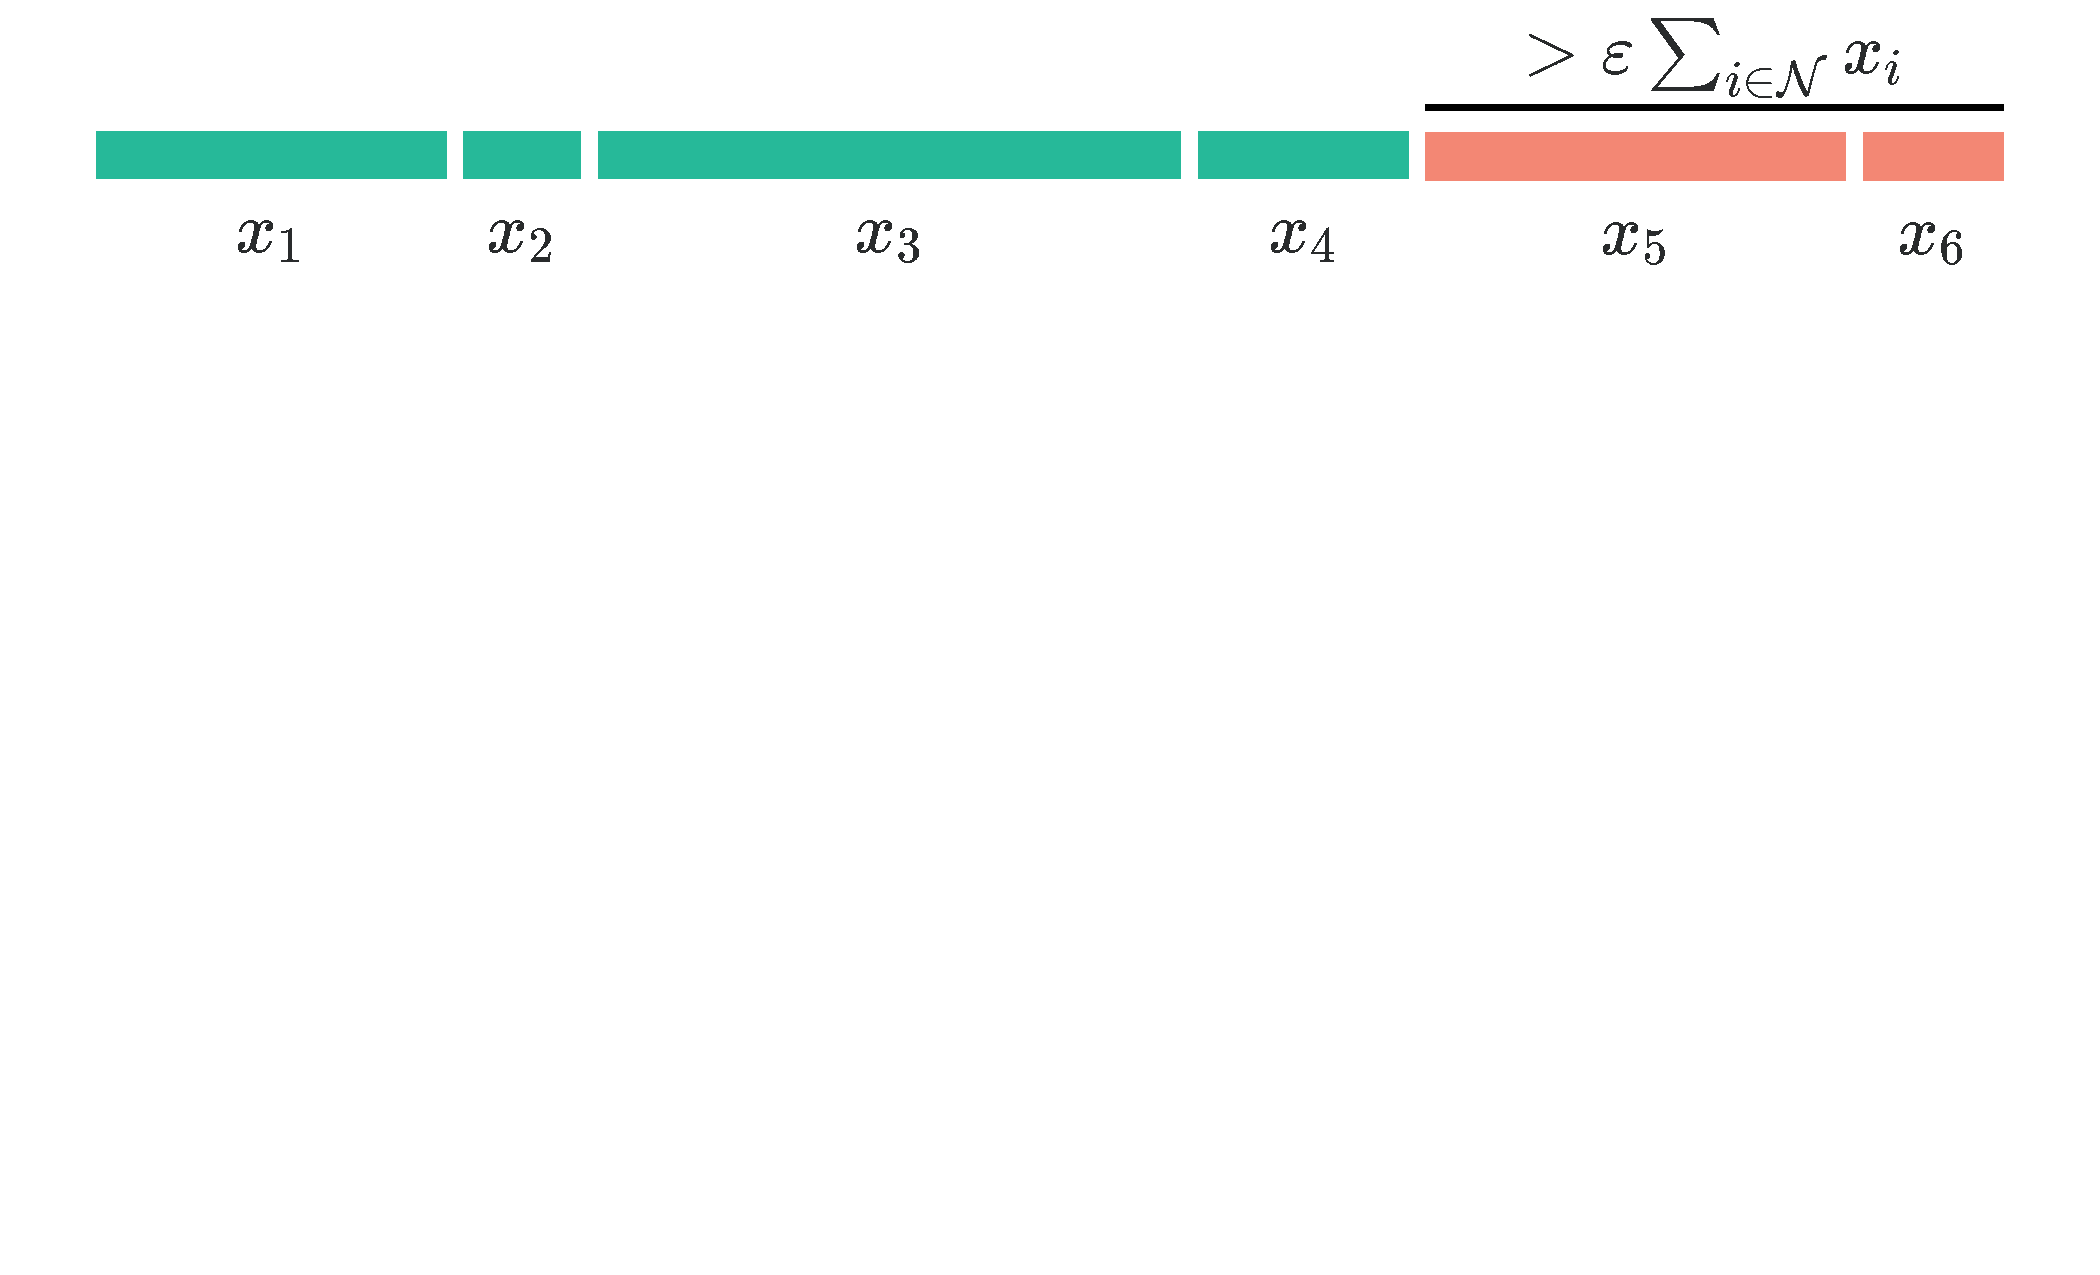
\includegraphics[clip, trim=1cm 17cm 2cm 0.2cm,width=0.65\textwidth]{figure4.pdf}}
  \caption{If the invalid records make up more than $\eps$ fraction of the total sum, there is at least $\eps$ probability that an invalid record is found with a single verification.}
\end{figure}


\begin{lemma}\label{lem:sumV}
Let $x_1, x_2, \dots, x_n \ge 0$ be the values of the records in $\Workers$ and $f(\xw) = \sum_{i \in \Workers} x_i$. Consider 
the probability distribution $p_i = \frac {x_i} {\sum_j x_j}$ which assigns to each record a probability proportional to its 
value $x_i$. Verifying $k=\Theta(\frac{1}{\eps}\log (1/\delta))$ records sampled independently from $p$, guarantees that the 
certification task succeeds with probability at least $1 - \delta$.
\end{lemma}

\begin{proof}
  Since $\Truth\subseteq \Workers$ and $x_i$'s are positive numbers, the inequality 
$\sum_{i \in \Workers} x_i \ge (1-\eps) \sum_{i \in \Truth} x_i$ holds trivially. If the inequality 
$\sum_{i \in \Workers} x_i \le \frac 1 {1-\eps} \sum_{i \in \Truth} x_i$ does not hold, we can bound the probability that all 
of the $k$ verifications fail to find an invalid record, as follows:

The probability that a single verification fails to find an invalid record is 
$\sum_{i \in \Truth} p_i = \frac {\sum_{i \in \Truth} x_i} {\sum_{i \in \Workers} x_i} < 1 - \eps.$

Therefore the probability that all $k$ verifications fail is at most $(1-\eps)^k$. Setting 
$k = \Theta(\frac{1}{\eps}\log (1/\delta))$, we guarantee that an invalid record is found with probability at least $1-\delta$.
\end{proof}

% !TeX root = main.tex

\subsection{Functions given by Linear Programs}
\label{ssubs:coverLP}

  We now extend the previous results for the sum function to more general objective functions that can be represented 
as linear programs. We first consider the special case of packing and covering LPs while later we present a result for
general linear programs.

$$
  \begin{array}{cc}
 	
\textbf{Packing LP} &
\textbf{Covering LP} \\
  
  \begin{array}{llll}
    \max_y  & \displaystyle\sum\limits_{i \in \Workers} c_{i} & y_{i} & \\
    \text{s.t.} & \displaystyle\sum\limits_{i \in \Workers} a_{ij} & y_{i} \le b_{j},  &j = 1, \dots, m \\
    & & y_i \ge 0, & i \in \Workers
  \end{array}
  
  &
  \begin{array}{llll}
      \min_x  & \displaystyle\sum\limits_{j = 1}^m b_{j} & x_{j} & \\
      \text{s.t.} & \displaystyle\sum\limits_{j = 1}^m a_{ij} & x_{j} \ge c_{i},  & i \in \Workers \\
      & & x_j \ge 0, & j = 1, \dots, m
    \end{array}
  \end{array}
$$

  Packing and Covering LP's are parameterized by the \emph{non-negative} parameters $a_{ij}, b_j, c_i$. We assume that
each record $i$ contains all parameters under his control, i.e. the value $c_i$ and $a_{ij}$ for all $j$, while the 
parameters $b_j$ are accurately known in advance.

  Packing LPs capture settings where several resources (each available in a quantity $b_j$) are to be divided among 
a set of agents in the system and agents report how much of each resource they need (given by $a_{ij}$) and how much
value they can generate if they are given the resources they ask for (given by $c_{ij}$). Our goal is to compute an
efficient allocation to agents that maximizes the total value generated. For the certification task, we want to 
certify that the total value generated by the true agents in an optimal allocation is close to the value computed 
under the possibly incorrect reports. We show that efficient certification schemes exist by extending the 
certification scheme presented for the sum function:

\begin{lemma} \label{lem:packingLP}
    Let $a_{ij}, c_i  \ge 0$ be values contained in the records $\Workers$ and $y^*$ be the optimal solution to the 
  packing LP. Consider the probability distribution $p_i = \frac {y^*_i c_i} {\sum_j y^*_j z_j}$ which assigns records 
  a probability proportional to their computed value $y^*_i c_i$. Verifying $k=\Theta(\frac{1}{\eps}\log (1/\delta))$ 
  records sampled independently from $p$, guarantees that the certification task for the packing LP succeeds with 
  probability at least $1 - \delta$.
\end{lemma}

  To see why this lemma holds, notice that the value $\sum_{i \in \Workers} c_i y^*_i$ computed using all the records 
$\Workers$ is higher than the value $\sum_{i \in \Truth} c_i \bar y_i$ computed using only the valid records $\Truth$. 
Moreover, if $\sum_{i \in \Truth} c_i y^*_i \ge (1-\eps) \sum_{i \in \Workers} c_i y^*_i$, then it must be that
$\sum_{i \in \Truth} c_i \bar y_i \ge (1-\eps) \sum_{i \in \Workers} c_i y^*_i$ as well, since setting $y_i = y^*_i$ 
for $i\in \Truth$ and $y_i=0$ otherwise is a feasible solution to the packing LP under the valid records. Finally, if  
$\sum_{i \in \Truth} c_i y^*_i < (1-\eps) \sum_{i \in \Workers} c_i y^*_i$, it means that invalid records contribute 
more than an $\eps$ fraction of the total value and thus an invalid record can be easily found as in the previous case
of the sum function.

  Covering LPs naturally capture various settings with public goods where the designer wants to introduce new goods to
satisfy all the demands coming from the records of our data set, but minimizing the total cost at the same time. In 
facility location problems, the designer wants to open facilities so that all a set of agents have access to at least
one facility and the agents report which locations are accessible to them.

  Certification schemes for covering LPs are less direct than previous examples, but can be easily obtained through LP 
duality. As the dual of a covering LP is a packing LP which has the \emph{exact same value}, we can use the certification 
scheme of Lemma~\ref{lem:packingLP} to certify that value. We directly get the following:

\begin{lemma} \label{lem:coveringLp}
    Let $a_{ij}, c_i \ge 0$ be values in the records $\Workers$. Verifying $k=\Theta(\frac{1}{\eps}\log (1/\delta))$ records 
  sampled independently according to a distribution $p$ given by the solution to the dual packing LP, guarantees that the 
  certification task for the covering LP succeeds with probability at least $1 - \delta$.
\end{lemma}

  General LPs can be written in the form of a packing or a covering LP but have arbitrary (possibly negative) parameters 
$a_{ij}, b_j, c_i$. The value of such LPs is harder to certify in general as a lot more verifications than before might be 
needed. However, we can show that $m$ verifications suffice to certify their value exactly.

\begin{lemma} \label{lem:generalLp}
    Let $a_{ij}, c_i$ be (possibly negative) values contained in the records $\Workers$. The certification complexity for 
  general LPs (written in the form of packing or covering LPs above) is at most $m$.
\end{lemma}

  To see why this is true, notice that in the covering LP formulation, the optimal value is given by at most $m$ tight 
constraints as there are only $m$ variables. Verifying the $m$ records relevant to those constraints guarantees that the 
optimal value of the LP under only the value of the records is equal to the computed one. This is because only those $m$ 
constraints determine the optimal value and even if every other constraint $i$ was dropped (i.e. because $i \notin \Truth$)
the value would remain the same. The result also holds for general LPs under the packing LP formulation by LP duality.



  % !TeX root = main.tex
\section{Certification Schemes for $\vec{w}$-Lipschitz Functions and Applications} \label{sec:instOpt}

    In this section, we present a unified way of finding \textit{almost-optimal certification schemes}. For a given
a function $f$, a desired approximation parameter $\eps$ and an instance $\vec{x}_{\Workers}$, we want to compute the
``instance-optimal'' number of verifications in order to certify that
$f(\vec{x}_{\Workers}) \in \left[ 1 - \eps, \frac{1}{1 - \eps} \right] f(\xt)$ with probability of failure at most $1/3$.
The first result of this section is a structural result. We show that even though optimal schemes may be arbitrarily
complex, there are simpler schemes, that verify records independently, which are almost-optimal.
\smallskip

To show this we define for every set $S\subseteq \Workers$ the probability $p_S$ that the instance-optimal certification scheme
$\mathcal{C}^*$ verifies at least one record in $S$, i.e. $p_S = \Prob\left(\bigcup_{i \in S} \text{ \{$\mathcal{C}^*$ verifies
record $i$\}} \right)$. For such an event, we say that the \emph{certification scheme verifies $S$} and for simplicity we denote
$p_i$, the probability that $\mathcal{C}^*$ verifies record $i$, i.e. $p_i = p_{\{i\}}$.

    For the instance $\vec{x}_\Workers$, the set of invalid records could be any $S \subseteq \Workers$. For the certification
scheme to work with failure probability at most $2/3$, we must have that $p_{S} \ge 2/3$ for any subset $S \subseteq \Workers$
such that $f(\xw)/f(\vec{x}_{\Workers\setminus S}) \notin [1 - \eps, 1/(1 - \eps)]$. If this doesn't hold for some $S$, an
adversary could choose the set of invalid records to be $S$ and the certification scheme $\mathcal{C}^*$ would fail with
probability more than $1/3$. Moreover, even though the  optimal certification scheme $\mathcal{C}^*$ may verify records in a very
correlated way, we have that  $\sum_{i \in  S} p_i \ge p_{ S} \ge 2/3$ from a simple union bound. Therefore, the certification
scheme $\mathcal{C}^*$ must satisfy the following set of necessary conditions:
  \[ \sum_{i \in  S} p_i \ge 2/3 ~~~\forall S \subseteq \Workers \text{~ such that ~} \frac{f(\xw)}{f(\vec{x}_{\Workers\setminus S})} \notin \left[ 1 - \eps, \frac{1}{1 - \eps} \right] \]

  \noindent By linearity of expectation, the expected total number of verifications that $\mathcal{C}^*$ performs is,
  \[ \Exp[ \text{total number of verifications} ] = \Exp \left[ \sum_{i \in \Workers} \vec{1}\text{\{$\mathcal{C}^*$ verifies record $i$\}} \right] = \sum_{i \in \Workers} p_i \] % TODO define \vec{1}

\noindent The above imply that the value of the following linear program is a lower bound on the total number of verifications
needed by the optimal scheme $\mathcal{C}^*$ for this specific instance $\vec{x}_\Workers$.
  \begin{equation}
    \label{eq:neccLP1}
    \begin{array}{ll@{}ll}
      \min  & \displaystyle\sum\limits_{i \in \Workers} & ~p_i & \\
      \text{s.t.} & \displaystyle\sum\limits_{i \in S} & ~p_i \ge 2/3, & \forall S \subseteq \Workers, \frac{f(\xw)}{f(\vec{x}_{\Workers\setminus S})} \notin \left[ 1 - \eps, \frac{1}{1 - \eps} \right] \\
                  & 0 \le & ~p_i \le 1, & \forall i \in \Workers
    \end{array}
  \end{equation}

  \noindent Notice that the solutions to LP~\eqref{eq:neccLP1}, do not directly correspond to certification schemes with success
probability $2/3$. However, as we show, any solution to LP \eqref{eq:neccLP1} can be converted to a certification scheme with
number of verifications at most twice as many as the optimal value of LP \eqref{eq:neccLP1} and success probability $2/3$. Since
the optimal value of LP \eqref{eq:neccLP1} lower bounds the instance optimal number of verifications, our derived certification
scheme will be a 2-approximation to the instance optimal scheme.

\begin{definition}
    For a solution $\bar{p}$ of LP~\eqref{eq:neccLP1}, we define the certification scheme $\mathcal{C}_{\bar{p}}$ that verifies
  each record $i$ independently with probability $q_i=\min\{2\bar{p}_i,1\}$.
\end{definition}

  It is clear that the certification scheme $\mathcal{C}_{\bar{p}}$ uses in expectation at most twice as many verifications as
the optimal value of LP~\eqref{eq:neccLP1} and the instance optimal scheme. We now show that it also achieves, success probability
of $2/3$ as required.
\medskip

\noindent Assume that the subset of valid records is $\Truth = \Workers \setminus S$. The probability that the scheme
$\mathcal{C}_{\bar{p}}$ does not verify anyone in the set $S = \{s_1, \dots, s_m\}$ is
\[ \Prob(\text{$\mathcal{C}_{\bar{p}}$ doesn't verify $\Truth$}) = \Prob( (\text{$\mathcal{C}_{\bar{p}}$ doesn't verify $s_1$}) \wedge \dots \wedge (\text{$\mathcal{C}_{\bar{p}}$ doesn't verify $s_m$})) =\prod_{s \in S} (1 - q_s) \]

\noindent Since $\bar{p}$ is a feasible solution to LP~\eqref{eq:neccLP1}, the probability that some record from $S$ is verified is

\[ \Prob(\text{$\mathcal{C}_{\bar{p}}$ verifies $S$}) = 1 - \prod_{s \in S} (1 - q_s) \ge 1 - \exp\left( - 2\sum_{i \in S} \bar{p}_s \right) \ge 1 - \exp\left( - 4/3 \right)\ge 2/3. \]
\noindent This means that our certification scheme succeeds with probability $2/3$ using at most twice the optimal number of
verifications in expectation. We can amplify the probability of $2/3$, making it arbitrarily close to one by repeating the
certification scheme. Since the repetitions are independent and each of them fails with probability at most $1/3$, after $r$
repetitions the total probability of failure is $3^{-r}$. Repeating $r = \log(1 / \delta)$ times, guarantees that for any
subset $S$, the probability that it will be verified is at least $1-\delta$. This result is summarized in the following theorem.
%\[ \Prob(\text{we verify $S$}) \ge 1 - \delta \]

%Therefore, solving LP~\eqref{eq:neccLP1}, we get a certification scheme that requires at most a factor of $\log(1 / \delta)$ more verifications than the instance optimal possible certification scheme.

\begin{theorem} \label{thm:optInstV}
    For any given function $f : \Domain^* \to \reals$ and any set of valus if records $\xw$, a solution to LP~\eqref{eq:neccLP1} corresponds to a
  certification scheme that verifies records of the data set independently using at most twice as many verifications as the optimal scheme for
  this instance and succeeds with probability $2/3$. Repeating the scheme $\log(1 / \delta)$ times increases the success probability to
  $1-\delta$.
\end{theorem}

\paragraph{Remark} We note that the LP~\eqref{eq:neccLP1} has exponentially many constraints and it may be computationally
intractable to solve depending on the function. It is very useful though as a tool to uncover the structure of approximately
optimal certification schemes. For example, Theorem \ref{thm:optInstV} implies that even though optimal schemes may be arbitrarily
complex, there are simpler schemes, that verify records independently, which are almost-optimal.
\medskip

In the following section, we derive a general methodology to obtain solutions to LP~\eqref{eq:neccLP1} for the very general class of
$\vec{w}$-Lipschitz functions.

\subsection{Certification Schemes for $\mathbf{w}$-Lipschitz Functions}

  In this section we show how we can use Theorem \ref{thm:optInstV} to get sufficient smoothness conditions on the function $f$
that can be used to provide certification schemes with small number of verifications.

  For any record $i \in \Workers$ we define $w_i$ to be the \textit{weight} of the record $i$. The weight of record $i$ will be
the quantity that will determine the probability that we will verify record $i$ according to the verification scheme that we want
to define. We state now the property that we want $f$ to satisfy in order to find a good verification scheme.

\begin{definition} \label{def:wcont}
  We say that a function $f : \Domain^* \to \reals$ is $\vec{w}$-\emph{Lipschitz}, with $\vec{w} \in \reals_+^n$, if for any
  $S \subseteq \Workers$ it holds that $|f(\xw) - f(\vec{x}_{\Workers\setminus S})| \le \sum_{i \in S} w_i$.
\end{definition}

\noindent For any function that satisfies this Lipschitz property we can get a good verification scheme that depends on the weight
vector $\vec{w}$.

\begin{theorem} \label{thm:wcont}
    For any non-negative $\vec{w}$-Lipschitz function $f : \Domain^* \to \reals_+$, set of records $\Workers$ with value $\xw$, and
  real numbers $\eps, \delta > 0$,
  \noindent there exists a certification scheme that uses at most
  $\frac{4\sum_{i \in \Workers} w_i}{3 f(\xw) \eps} \log(1 / \delta) $
  verifications and has probability of success at least $1 - \delta$.
\end{theorem}


%\subsection{Minimum Spanning Tree}
\label{ssec:mstIOpt}


  In Appendix \ref{sec:app:proofOfLipschitz} we present the proof of Theorem \ref{thm:wcont}. Also, in Appendix \ref{ssec:tspIOpt} and \ref{ssec:steinerIOpt}, we present two applications of Theorem \ref{thm:wcont} to get
certification schemes for the \emph{Traveling Salesman (TSP)} and the \emph{Steiner Tree} problems. In both applications, we show that
the optimal solution is $\vec{w}$-Lipschitz with $\frac{\sum_{i \in \Workers} w_i}{f(\xw)} \le 2$. Hence, the total number of
verifications by Theorem \ref{thm:wcont} is $O((1/\eps) \log(1/\delta))$.


  % !TeX root = main.tex
\section{Weak Correction Model}
\label{sec:wcorr}

  We show how starting from a certification scheme, we can obtain a weak-correction scheme with the same verification complexity
(up to constants).

\begin{theorem}\label{thm:reduction}
    Suppose that there exists a certification scheme for a function $f$ that uses $q(n,\eps)$ verifications and fails with probability $1/3$. Then,
  there exists a weak-correction scheme with verification complexity $O(q(n,\eps) \log(1/\delta))$ that outputs an accurate estimate of the function
  $f$ and fails with  probability $\delta$.
\end{theorem}


%\textcolor{red}{Initially, we are going to assume (for simplicity) that the function $f$ that we want to approximate is increasing. That is, if an incorrect input is removed the approximation of the answer can only get better. However, in the next section we show that this assumption is not necessary. }

  Theorem \ref{thm:reduction} shows that the certification task we defined in section \ref{sec:certification} is already strong enough to perform this
seemingly more challenging task. Intuitively, this is because we can run many rounds of certification until we have enough confidence that we have an
accurate result while we remove from the dataset any invalid record we might find during these rounds. Indeed, a simple way to make the conversion
is to start from a certification scheme with error probability 1/3 and reduce its probability of error to $\delta/n$, by repeating it $\log(n/\delta)$
times. Then use this scheme repeatedly until no more invalid records are detected. By a union bound, the probability of error is at most $\delta$ since
the process takes at most $n$ steps.
  Theorem \ref{thm:reduction} shows a stronger result than the above result showing that the logarithmic dependence on the number of records can be avoided
if the stopping time is more carefully chosen. The full proof of Theorem~\ref{thm:reduction} is presented in Appendix~\ref{app:weak}.


  % !TeX root = main.tex
\section{Strong Correction Model} \label{sec:scorr}

  In section, we show that it is possible to obtain more efficient correction schemes for several problems. 
  We show that this is true for the sum function which implies strong correction schemes for other functions such as the average. 
  In addition, we show strong correction schemes for more general combinatorial tasks through a connection with conditional sampling.
  However, as we show there are 
simple functions, e.g. the composition of the max and the sum function, for which good weak correction schemes exist that do not admit strong correction schemes.

\subsection{Computing the Sum of Values of Records}

 Using the formulation in Section \ref{ssec:certificationSum}, we get the following result. Its proof appears in Appendix \ref{sec:app:scorr} and shows that $\Theta(1/\eps^2)$ verifications are both necessary and sufficient.

  
\begin{lemma} \label{lem:sumC}
    Let $x_1, x_2, \dots, x_n \ge 0$ be the values of the records $\Workers$ and $f(\xw) = \sum_{i \in \Workers} x_i$.
  Consider the probability distribution $p_i = \frac {x_i} {\sum_j x_j}$ which selects a record $x_i$ with probability 
  proportional to its value. If we sample $M$ times independently from $p$ until 
  $k = \Theta\left(\frac{1}{\eps^2}\log (1/\delta)\right)$ valid records found, then the estimator 
  $\hat{s} = \frac{k}{M} \sum_{i \in \Workers} x_i$ lies in
  $\left[ 1 - \eps, \frac{1}{1 - \eps} \right] \cdot \sum_{i \in \Truth} x_i$ w.p. at least $1 - \delta$. 
\end{lemma}


\subsection{Lower Bound for the Maximum of Sums Function}

  In this section we show that no efficient strong correction scheme exists for the composition of the max and the sum function. 
More precisely we assume we have a partition $\mathcal{J} = \{\Workers_1, \dots, \Workers_{\ell}\}$ of the set $\Workers$ and we 
want a strong correction scheme for the function $f(\xw) = \max_{A \in \mathcal{J}} \sum_{i \in A} x_i$. Lemma \ref{lem:maxOfSumC} shows that any strong 
correction scheme for $f$ that achieves constant approximation has to verify at least a constant fraction of the records. Its proof can be found in Appendix \ref{sec:app:scorr}. 

\begin{lemma} \label{lem:maxOfSumC}
    Let $c >0$. There exists a partition $\mathcal{J} = \{\Workers_1, \dots, \Workers_{\ell}\}$ of
  $\Workers$ and a vector $\xw \in \reals^n$ such that any strong correction scheme for the function 
  $f(\xw) = \max_{A \in \mathcal{J}} \sum_{i \in A} x_i$, that returns an estimate 
  $\hat{s} \in \left[\frac{1}{c}, c\right] \cdot f(\xt)$ with probability at least $3/4$, must verify
  $\abs{\Workers} / 4 c^2$ records.
\end{lemma}



\subsection{From Algorithms using Conditional Sampling to Strong Correction Schemes}

  The design of a strong correction scheme can be challenging since the guarantee is very strong. Our main theorem 
in this section shows that there is a correspondence of strong correction schemes with 
\textit{sublinear algorithms using conditional sampling}, introduced recently in \cite{GouleakisTZ2017}. We state here the main
theorem for this section and we defer its proof and applications for Appendix \ref{sec:app:applicationsStrongCorrection}.

\begin{theorem} \label{thm:sCorrection}
    Any function that can be approximated using $k$ conditional samples admits a strong correction scheme with cost $k$.
\end{theorem}

  \section*{Acknowledgements}
  The authors were supported by NSF CCF-1551875, CCF-1617730, CCF-1733808, and
  IIS-1741137.

  \bibliography{ZAMPETAKIS18}

  \appendix
  \clearpage
  \appendix

\section{Proof of Lemma \ref{thm:general_instantaneous}}
\begin{proof}{\textbf{of Lemma \ref{thm:general_instantaneous}}.}
We first state a useful property used in typical OMD analysis. Let $\Omega$ be a convex compact set in $\mathbb{R}^K$, $\psi$ be a convex function on $\Omega$, 
$w'$ be an arbitrary point in $\Omega$, and $x \in \mathbb{R}^K$.
If $w^*=\argmin_{w\in \Omega}\{\inn{w,x}+D_{\psi}(w,w')\}$, then for any $u \in \Omega$,
\begin{align*}
\inn{w^*-u, x}\leq D_{\psi}(u,w')-D_\psi(u,w^*)-D_{\psi}(w^*,w'). 
\end{align*}
This is by the first-order optimality condition of $w^*$ and direct calculations. Applying this to update rule~\eqref{eqn:update_rule_2} we have
\begin{align}
\inn{w_{t+1}^\p-u, \hat{\ell}_t+ a_t} \leq D_{\psi_t}(u,w_{t}^\p)-D_{\psi_t}(u,w_{t+1}^\p)-D_{\psi_t}(w_{t+1}^\p, w_{t}^\p); \label{eqn:apply1}
\end{align}
while applying it to update rule~\eqref{eqn:update_rule_1} and picking $u=w_{t+1}^\p$ we have
\begin{align}
\inn{w_t-w_{t+1}^\p, m_t} \leq D_{\psi_t}(w_{t+1}^\p, w_t^\p)-D_{\psi_t}(w_{t+1}^\p, w_t)-D_{\psi_t}(w_t, w_t^\p).\label{eqn:apply2} 
\end{align}
Now we bound the instantaneous regret as follows:
\begin{align}
&\inn{w_t-u, \hat{\ell}_t}\nonumber \\
&=\inn{w_t-u, \hat{\ell}_t+ a_t}-\inn{w_t, a_t}+\inn{u,  a_t}\nonumber \\
&=\inn{w_t-w_{t+1}^\p, \hat{\ell}_t+a_t}-\inn{w_t, a_t}+\inn{w_{t+1}^\p-u, \hat{\ell}_t+a_t}+\inn{u,   a_t}\nonumber \\
&=\inn{w_t-w_{t+1}^\p, \hat{\ell}_t+a_t-m_t}-\inn{w_t,a_t}+\inn{w_{t+1}^\p-u, \hat{\ell}_t+ a_t}+\inn{w_t-w_{t+1}^\p, m_t}+\inn{u,   a_t} \nonumber \\
&\leq D_{\psi_t}(u,w_{t}^\p)-D_{\psi_t}(u,w_{t+1}^\p)-D_{\psi_t}(w_{t+1}^\p, w_t)-D_{\psi_t}(w_t, w_t^\p)+\inn{u, a_t}, \label{eqn:regret_decomposition}
\end{align}
where last inequality is by the condition $\inn{w_t-w_{t+1}^\p, \hat{\ell}_t+a_t-m_t}-\inn{w_t,a_t}\leq 0$, Eq.~\eqref{eqn:apply1}, and Eq.~\eqref{eqn:apply2}.
\end{proof}

\section{Lemmas for Log-barrier OMD}
\label{section:all_kinds_of_lemmas}

In this section we establish some useful lemmas for update rules~\eqref{eqn:update_rule_1} and~\eqref{eqn:update_rule_2} with log-barrier regularizer,
which are used in the proofs of other theorems.
We start with some definitions.

\begin{definition}
\label{definition:norm}
For any $h \in \mathbb{R}^K$, define norm $\norm{h}_{t,w}=\sqrt{h^\top \nabla^2 \psi_t(w) h}=\sqrt{\sum_{i=1}^K \frac{1}{\eta_{t,i}}\frac{h_i^2}{w_i^2}}$ and its dual norm $\norm{h}_{t,w}^*=\sqrt{h^\top \nabla^{-2} \psi_t(w) h}=\sqrt{\sum_{i=1}^K \eta_{t,i}w_i^2 h_i^2}$.
For some radius $r > 0$, define ellipsoid $\mathcal{E}_{t,w}(r)=\left\{u \in \mathbb{R}^K : \norm{u-w}_{t,w}\leq r \right\}$ . 
\end{definition}

\begin{lemma}
\label{lemma:norm_close}
If $w^\p \in \mathcal{E}_{t,w}(1)$ and $\eta_{t,i}\leq \frac{1}{81}$ for all $i$, then $w_i^\p\in \left[ \frac{1}{2}w_i, \frac{3}{2}w_i \right]$ for all $i$, and also $ 0.9\norm{h}_{t,w} \leq \norm{h}_{t,w^\p} \leq 1.2\norm{h}_{t,w}$ for any $h\in \mathbb{R}^K$. 
\end{lemma}
\begin{proof}
$w^\p\in \mathcal{E}_{t,w}(1)$ implies $\sum_{i=1}^K \frac{1}{\eta_{t,i}}\frac{(w^\p_i-w_i)^2}{w_i^2}\leq 1$. Thus for every $i$, we have $\frac{\abs{w_i^\p-w_i}}{w_i}\leq \sqrt{\eta_{t,i}}\leq \frac{1}{9}$, implying $w_i^\p\in \left[ \frac{8}{9}w_i, \frac{10}{9}w_i \right]\subset\left[ \frac{1}{2}w_i, \frac{3}{2}w_i \right]$. 
Therefore, $\norm{h}_{t,w^\p}
=\sqrt{\sum_{i=1}^K \frac{1}{\eta_{t,i}} \frac{h_i^2}{w^{\p 2}_i}}
\geq \sqrt{\sum_{i=1}^K \frac{1}{\eta_{t,i}}\frac{h_i^2}{\left(\frac{10}{9}w_i\right)^2}}
=0.9\norm{h}_{t,w}$. 
Similarly, we have $\norm{h}_{t,w^\p}\leq 1.2\norm{h}_{t,w}$. 
\end{proof}

\begin{lemma}
\label{lemma:stability}
Let $w_t, w_{t+1}^\p$ follow \eqref{eqn:update_rule_1} and \eqref{eqn:update_rule_2} where $\psi_t$ is the log-barrier with $\eta_{t,i}\leq \frac{1}{81}$ for all $i$. If $\norm{\hat{\ell}_t-m_t+a_t}^*_{t,w_t}\leq \frac{1}{3}$, then $w_{t+1}^\p \in \mathcal{E}_{t,w_t}(1)$. 
\end{lemma}

\begin{proof}
Define $F_{t}(w)=\inn{w, m_t}+D_{\psi_t}(w, w_t^\p)$ and $F_{t+1}^\p(w)=\inn{w, \hat{\ell}_t+a_t}+D_{\psi_t}(w, w_t^\p)$. Then by definition we have $w_t=\argmin_{w\in\Omega}F_{t}(w)$ and $w_{t+1}^\p=\argmin_{w\in\Omega}F_{t+1}^\p(w)$. To show $w_{t+1}^\p\in \mathcal{E}_{t,w_t}(1)$, it suffices to show that for all $u$ on the boundary of $\mathcal{E}_{t,w_t}(1)$, $F^\p_{t+1}(u)\geq F^\p_{t+1}(w_t)$. 

Indeed, using Taylor's theorem, for any $u\in \partial \mathcal{E}_{t,w_t}(1)$, there is an $\xi$ on the line segment between $w_t$ and $u$ such that (let $h\triangleq u-w_t$)
\begin{align*}
F^\p_{t+1}(u)&=F^\p_{t+1}(w_t)+\nabla F^{\p}_{t+1} (w_t)^\top h+ \frac{1}{2}h^\top\nabla^2 F^\p_{t+1}(\xi)h \\
&=F^\p_{t+1}(w_t)+ (\hat{\ell}_t-m_t+a_t)^\top h +\nabla F_t (w_t)^\top h+ \frac{1}{2}h^\top\nabla^2 \psi_t(\xi)h \\
&\geq F^\p_{t+1}(w_t)+ (\hat{\ell}_t-m_t+a_t)^\top h + \frac{1}{2}\norm{h}_{t,\xi}^2 \tag{by the optimality of $w_t$}\\
&\geq F^\p_{t+1}(w_t)+ (\hat{\ell}_t-m_t+a_t)^\top h + \frac{1}{2}\times0.9^2\norm{h}_{t,w_t}^2 \tag{by Lemma \ref{lemma:norm_close}} \\
&\geq F^\p_{t+1}(w_t)- \norm{\hat{\ell}_t-m_t+a_t}^*_{t,w_t} \norm{h}_{t,w_t} + \frac{1}{3}\norm{h}_{t,w_t}^2 \\
&=F^\p_{t+1}(w_t)- \norm{\hat{\ell}_t-m_t+a_t}^*_{t,w_t} + \frac{1}{3} \tag{$\norm{h}_{t,w_t}=1$}\\
&\geq F^\p_{t+1}(w_t). \tag{by the assumption}
\end{align*}
\end{proof}

\begin{lemma}
\label{lemma:stability_under_condition}
Let $w_t, w_{t+1}^\p$ follow \eqref{eqn:update_rule_1} and \eqref{eqn:update_rule_2} where $\psi_t$ is the log-barrier with $\eta_{t,i}\leq \frac{1}{81}$ for all $i$. If $\norm{\hat{\ell}_t-m_t+a_t}^*_{t,w_t}\leq \frac{1}{3}$, then $\norm{w_{t+1}^\p-w_t}_{t,w_t}\leq 3\norm{\hat{\ell}_t-m_t+a_t}_{t,w_t}^*$. 
\end{lemma}
\begin{proof}
Define $F_t(w)$ and $F_{t+1}^\p(w)$ to be the same as in Lemma \ref{lemma:stability}. Then we have 
\begin{align}
F_{t+1}^\p(w_t)-F_{t+1}^\p(w_{t+1}^\p)&=(w_t-w_{t+1}^\p)^\top(\hat{\ell}_t-m_t+a_t) + F_t(w_t)-F_t(w_{t+1}^\p) \nonumber \\
&\leq (w_t-w_{t+1}^\p)^\top(\hat{\ell}_t-m_t+a_t) \nonumber \tag{optimality of $w_t$}\\
&\leq \norm{w_t-w_{t+1}^\p}_{t,w_t}\norm{\hat{\ell}_t-m_t+a_t}_{t,w_t}^*. \label{eqn:direction1}
\end{align}
On the other hand, for some $\xi$ on the line segment between $w_t$ and $w_{t+1}^\p$, we have by Taylor's theorem and the optimality of $w_{t+1}^\p$,
\begin{align}
F_{t+1}^\p(w_t)-F_{t+1}^\p(w_{t+1}^\p)&=\nabla F_{t+1}^\p(w_{t+1}^\p)^\top (w_t-w_{t+1}^\p) + \frac{1}{2}(w_t-w_{t+1}^\p)^\top \nabla^2 F_{t+1}^\p(\xi)(w_t-w_{t+1}^\p) \nonumber \\
&\geq \frac{1}{2}\norm{w_t-w_{t+1}^\p}_{t,\xi}^2 .
\label{eqn:direction2}
\end{align}
Since the condition in Lemma \ref{lemma:stability} holds, $w_{t+1}^\p\in \mathcal{E}_{t,w_t}(1)$, and thus $\xi\in \mathcal{E}_{t,w_t}(1)$. Using again Lemma \ref{lemma:norm_close}, we have 
\begin{align}
\frac{1}{2}\norm{w_t-w_{t+1}^\p}_{t,\xi}^2 \geq \frac{1}{3}\norm{w_t-w_{t+1}^\p}_{t,w_t}^2\label{eqn:direction3}.
\end{align}
Combining \eqref{eqn:direction1}, \eqref{eqn:direction2}, and \eqref{eqn:direction3}, we have $\norm{w_t-w_{t+1}^\p}_{t,w_t}\norm{\hat{\ell}_t-m_t+a_t}_{t,w_t}^* \geq \frac{1}{3}\norm{w_t-w_{t+1}^\p}_{t,w_t}^2$, which leads to the stated inequality. 
\end{proof}

\begin{lemma}
\label{lemma:condition_automatic_hold}
%Let $w_t, w_{t+1}^\p$ follow \eqref{eqn:update_rule_1} and \eqref{eqn:update_rule_2}. 
When the three conditions in Theorem \ref{lemma:MAB_condition} hold, we have $\norm{\hat{\ell}_t-m_t+a_t}^{*}_{t,w_t}\leq \frac{1}{3}$ for either $a_{t,i}=6\eta_{t,i}w_{t,i}(\hat{\ell}_{t,i}-m_{t,i})^2$ or $a_{t,i}=0$.  
\end{lemma}
\begin{proof}
For $a_{t,i}=6\eta_{t,i}w_{t,i}(\hat{\ell}_{t,i}-m_{t,i})^2$, we have
\begin{align*}
\norm{\hat{\ell}_t-m_t+a_t}^{*2}_{t,w_t}
&= \sum_{i=1}^K\eta_{t,i}w_{t,i}^2\big(\hat{\ell}_{t,i}-m_{t,i} + 6\eta_{t,i}w_{t,i}(\hat{\ell}_{t,i}-m_{t,i})^2\big)^2 \\
&=\sum_{i=1}^K\eta_{t,i}w_{t,i}^2(\hat{\ell}_{t,i}-m_{t,i})^2+12\eta_{t,i}^2w_{t,i}^3(\hat{\ell}_{t,i}-m_{t,i})^3 +36\eta_{t,i}^3w_{t,i}^4(\hat{\ell}_{t,i}-m_{t,i})^4\\
&\leq \sum_{i=1}^K \eta_{t,i}w_{t,i}^2(\hat{\ell}_{t,i}-m_{t,i})^2(1+36\eta_{t,i}+324\eta_{t,i}^2) \tag{condition (ii)}\\
&\leq 2\sum_{i=1}^K \eta_{t,i}w_{t,i}^2(\hat{\ell}_{t,i}-m_{t,i})^2 \tag{condition (i)}\\
&\leq 2\times \frac{1}{18}=\frac{1}{9}.\tag{condition (iii)}
\end{align*}
For $a_{t,i}=0$, we have
\begin{align*}
\norm{\hat{\ell}_t-m_t+a_t}^{*2}_{t,w_t}=\norm{\hat{\ell}_t-m_t}^{*2}_{t,w_t}=\sum_{i=1}^K \eta_{t,i}w_{t,i}^2(\hat{\ell}_{t,i}-m_{t,i})^2\leq \frac{1}{18} < \frac{1}{9}. \tag{condition (iii)}
\end{align*}
%When $a_{t,i}=0$,
%\begin{align*}
%\norm{\hat{\ell}_t-m_t+a_t}_{t,w_t}^{*2}= \sum_{i=1}^K \eta_{t,i}w_{t,i}^2(\hat{\ell}_{t,i}-m_{t,i})^2 \leq \frac{1}{18}<\frac{1}{9}. \text{\ \ \ \ \ \ \ \ \ \ \ \ \ \ \ \ \ \ \ \ \ \ \ (condition(iii))} 
%\end{align*}
\end{proof}

\begin{lemma}
\label{lemma:2times_bound}
If the three conditions in Theorem \ref{lemma:MAB_condition} hold, \textsc{Broad-OMD} (with either Option I or II)
satisfies $\frac{1}{2}w_{t,i}\leq w^\p_{t+1,i}\leq \frac{3}{2}w_{t,i}$.
%Let $w_t, w_{t+1}^\p$ follow \eqref{eqn:update_rule_1} and \eqref{eqn:update_rule_2}. If the three conditions in Theorem \ref{lemma:MAB_condition} hold, then $\frac{1}{2}w_{t,i}\leq w^\p_{t+1,i}\leq \frac{3}{2}w_{t,i}$, for either $a_{t,i}=6\eta_{t,i}w_{t,i}(\hat{\ell}_{t,i}-m_{t,i})^2$ or $a_{t,i}=0$.
\end{lemma}
\begin{proof}
This is a direct application of Lemmas \ref{lemma:condition_automatic_hold},  \ref{lemma:stability}, and \ref{lemma:norm_close}.
%It suffices to prove $w_{t+1}^\p \in \mathcal{E}_{t,w_t}(1)$, because if it is true, then
%\begin{align*}
%\norm{w_{t+1}^\p-w_t}_{t,w_t}=\sqrt{\sum_{i=1}^K\frac{1}{\eta_{t,i}}\frac{(w^\p_{t+1,i}-w_{t,i})^2}{w_{t,i}^2}}\leq 1, 
%\end{align*}
%which implies $\frac{\abs{w_{t+1,i}^\p-w_{t,i}}}{w_{t,i}}\leq \sqrt{\eta_{t,i}}\leq \frac{1}{2}$. Thus, $w_{t+1,i}^\p \in [\frac{1}{2}w_{t,i}, \frac{3}{2}w_{t,i}]$.

%Since we assume the three conditions in Theorem \ref{lemma:MAB_condition} hold, $w_{t+1}^\p \in \mathcal{E}_{t,w_t}(1)$ can be proved by applying Lemma \ref{lemma:condition_automatic_hold} and Lemma \ref{lemma:stability} back to back.

\end{proof}

\begin{lemma}
\label{lemma:2times_bound_another}
For the MAB problem, if the three conditions in Theorem \ref{lemma:MAB_condition} hold, \textsc{Broad-OMD} (with either Option I or II)
satisfies $\frac{1}{2}w_{t,i}\leq w^\p_{t,i}\leq \frac{3}{2}w_{t,i}$.
\end{lemma}
\begin{proof}
It suffices to prove $w_{t}^\p \in \mathcal{E}_{t,w_t}(1)$ by Lemma~\ref{lemma:norm_close}.
Since we assume that the three conditions in Theorem \ref{lemma:MAB_condition} hold and $w_t\in \Delta_K$, we have $\norm{m_t}_{t,w_t}^*=\sqrt{\sum_{i=1}^K \eta_{t,i}w_{t,i}^2m_{t,i}^2}\leq \sqrt{\frac{1}{162}\sum_{i=1}^K w_{t,i}^2}\leq \sqrt{\frac{1}{162}}< \frac{1}{3}$. This implies $w_{t}^\p \in \mathcal{E}_{t,w_t}(1)$ by a similar arguments as in the proof of Lemma~\ref{lemma:stability} (one only needs to replace $F_{t+1}^\p(w)$ there by $G(w)\triangleq D_{\psi_t}(w,w_t^\p)$ and note that $w_t^\p=\argmin_{w\in \Delta_K}G(w)$).
\end{proof}


%\begin{lemma}
%\label{lemma:stability_game}
%For MAB problems, if the three conditions in Theorem \ref{lemma:MAB_condition} hold, then \textsc{Broad-OMD} with $a_{t,i}=\mathbf{0}$ and fixed learning rate $\eta$ guarantees $\norm{w_{t+1}-w_t}_1 = \mathcal{O}(\eta)$ for all $t$.  
%\end{lemma}
%\begin{proof}
%By Lemma \ref{lemma:condition_automatic_hold} and \ref{lemma:stability_under_condition}, we have $\norm{w_t-w_{t+1}^\p}_{t,w_t}\leq 3\norm{\hat{\ell}_t-m_t}_{t,w_t}^*$, which implies
%\begin{align*}
%\frac{1}{\eta}\frac{(w_{t,j}-w_{t+1,j}^\p)^2}{w_{t,j}^2}\leq \sum_{i=1}^K\frac{1}{\eta}\frac{(w_{t,i}-w_{t+1,i}^\p)^2}{w_{t,i}^2}\leq 3\eta\sum_{i=1}^K  w_{t,i}^2(\hat{\ell}_{t,i}-m_{t,i})^2\leq 3\eta\times 9. 
%\end{align*}
%Therefore, $\abs{w_{t,j}-w_{t+1,j}^\p} = \mathcal{O}(\eta w_{t,j})$. We can use similar techniques in Lemma \ref{lemma:condition_automatic_hold} and \ref{lemma:stability_under_condition} to prove $\norm{w_{t+1}-w_{t+1}^\p}_{t,w_{t+1}^\p}\leq 3\norm{m_{t+1}}_{t,w_{t+1}^\p}^*$, and thus  $\abs{w_{t+1,j}^\p-w_{t+1,j}}=\mathcal{O}(\eta w_{t+1,j}^\p)=\mathcal{O}(\eta w_{t,j})$. Thus, $\abs{w_{t,j}-w_{t+1,j}}=\mathcal{O}(\eta w_{t,j})$, which implies $\norm{w_t-w_{t+1}}_1=\mathcal{O}(\eta)$. 
%\end{proof}

\section{Proof of Theorem \ref{lemma:MAB_condition} and Corollary~\ref{cor:clear_corollary}}
%To prove Theorem \ref{lemma:MAB_condition}, we need some definitions and lemmas established in Section~\ref{section:all_kinds_of_lemmas}. 

\begin{proof}{\textbf{of Theorem \ref{lemma:MAB_condition}}.}
We first prove Eq.~\eqref{eqn:condition1} holds: by Lemmas \ref{lemma:condition_automatic_hold} %, we have $\norm{\hat{\ell}_t-m_t+a_t}^{*}_{t,w_t}\leq \frac{1}{3}$. Then by
and \ref{lemma:stability_under_condition}, we have
\begin{align*}
\inn{w_t-w_{t+1}^\p, \hat{\ell}_t-m_t+ a_t}
&\leq \norm{w_t-w_{t+1}^\p}_{t,w_t}\norm{\hat{\ell}_t-m_t+a_t}_{t,w_t}^*\\
&\leq 3\norm{\hat{\ell}_t-m_t+a_t}_{t,w_t}^{*2}\\
&\leq 3\sum_{i=1}^K \eta_{t,i}w_{t,i}^2(\hat{\ell}_{t,i}-m_{t,i})^2(1+36\eta_{t,i}+324\eta_{t,i}^2) \\
&\leq 6\sum_{i=1}^K \eta_{t,i}w_{t,i}^2(\hat{\ell}_{t,i}-m_{t,i})^2 = \inn{w_t, a_t},
\end{align*}
where the last two inequalities are by the same calculations done in the proof of Lemma~\ref{lemma:condition_automatic_hold}.
%where $C=6$. With our choice of $C$ and $\eta_{t,i}$, we have $3(1+6\eta_{t,i}C+9\eta_{t,i}^2C^2)\leq 3\left(1+6\times\frac{6}{162}+9\times \left(\frac{6}{162}\right)^2\right)\leq C$. Therefore, the last expression is further bounded by $\sum_{i=1}^K C\eta_{t,i}w_{t,i}^2(\hat{\ell}_{t,i}-m_{t,i})^2$, which is equal to $\inn{w_t, a_t}$. 

Since Eq.~\eqref{eqn:condition1} holds, using Lemma~\ref{thm:general_instantaneous} we have (ignoring non-positive terms $-A_t$'s),
\begin{align}
\sum_{t=1}^T\inn{w_t-u, \hat{\ell}_t}&\leq \sum_{t=1}^T\left(D_{\psi_t}(u,w_t^\p)-D_{\psi_t}(u,w^\p_{t+1})\right)+\sum_{t=1}^T\inn{u,a_t}\nonumber \\
&\leq D_{\psi_1}(u, w_1^\p) + \sum_{t=1}^{T}\left( D_{\psi_{t+1}}(u, w^\p_{t+1})-D_{\psi_{t}}(u, w^\p_{t+1}) \right)+\sum_{t=1}^T\inn{u,a_t}.\label{eqn:some_intermediate}
\end{align}
In the last inequality, we add a term $D_{\psi_{T+1}}(u, w_{T+1}^\p) \geq 0$ artificially. As mentioned, $\psi_{T+1}$, defined in terms of $\eta_{T+1,i}$, never appears in the \textsc{Broad-OMD} algorithm. We can simply pick any $\eta_{T+1,i} > 0$ for all $i$ here. This is just to simplify some analysis later. 

The first term in \eqref{eqn:some_intermediate} can be bounded by the optimality of $w_1^\p$:
\begin{align*}
D_{\psi_1}(u, w_1^\p)&=\psi_1(u)-\psi_1(w_1^\p)-\inn{\nabla\psi_1(w_1^\p), u-w_1^\p}\\
&\leq \psi_1(u)-\psi_1(w_1^\p)=\sum_{i=1}^K \frac{1}{\eta_{1,i}}\ln\frac{w_{1,i}^\p}{u_i}.
\end{align*}
%where the inequality is because $w_1^\p$ is the minimizer of $\psi_1$. 
The second term, by definition, is
\begin{align*}
\sum_{t=1}^{T}\sum_{i=1}^K \left(\frac{1}{\eta_{t+1,i}}-\frac{1}{\eta_{t,i}}\right) h\left(\frac{u_i}{w_{t+1,i}^\p}\right). 
\end{align*}
Plugging the above two terms into \eqref{eqn:some_intermediate} finishes the proof.
\end{proof}

\begin{proof}{\textbf{of Corollary~\ref{cor:clear_corollary}}.}
We first check the three conditions in Theorem~\ref{lemma:MAB_condition} under our choice of $\eta_{t,i}$ and $\hat{\ell}_{t,i}$: $\eta_{t,i}=\eta=\frac{1}{162K_0}\leq \frac{1}{162}$; $w_{t,i}\abs{\hat{\ell}_{t,i}-m_{t,i}}=\abs{\ell_{t,i}-m_{t,i}}\mathbbm{1}\{i\in b_t\} \leq 2<3$; 
$\sum_{i=1}^K \eta_{t,i}w_{t,i}^2(\hat{\ell}_{t,i}-m_{t,i})^2=\frac{1}{162K_0}\sum_{i=1}^K (\ell_{t,i}-m_{t,i})^2\mathbbm{1}\{i\in b_t\} \leq \frac{4}{162} < \frac{1}{18}$. 
%(in the MAB case, $\sum_{i=1}^K \eta_{t,i}w_{t,i}^2(\hat{\ell}_{t,i}-m_{t,i})^2=\eta_{t,i_t}(\ell_{t,i_t}-m_{t,i_t})^2\leq \frac{1}{162}\times 3^2=\frac{1}{18}$). 
Applying Theorem~\ref{lemma:MAB_condition} we then have 
\begin{align*}
\sum_{t=1}^T \inn{w_t-u, \hat{\ell}_t}\leq \sum_{i=1}^K  \frac{\ln\frac{w^\p_{1,i}}{u_i}}{\eta}  +\sum_{t=1}^T \inn{u,a_t}.
\end{align*}
As mentioned, if we let $u=b^*$, then $\ln \frac{w_{1,i}^\p}{u_i}$
becomes infinity for those $i\notin b^*$. Instead, we let $u=\left(1-\frac{1}{T}\right)b^* + \frac{1}{T}w_1^\p$. With this choice of $u$, we have $\frac{w_{1,i}^\p}{u_i}\leq \frac{w_{1,i}^\p}{\frac{1}{T}w_{1,i}^\p}=T$. Plugging $u$ into the above inequality and rearranging, we get 
\begin{align}
\sum_{t=1}^T \inn{w_t-b^*, \hat{\ell}_t}\leq \frac{K\ln T}{\eta}+\sum_{t=1}^T \inn{b^*,a_t}+B,  \label{eqn:sb_corollary}
\end{align}
where $B\triangleq \frac{1}{T}\sum_{t=1}^T \inn{-b^*+w_1^\p, \hat{\ell}_t+a_t}$. 

Now note that $\mathbb{E}_{b_t}[a_{t,i}]=6\eta (\ell_{t,i}-m_{t,i})^2=\mathcal{O}(\eta)$ and $\mathbb{E}_{b_t}[\hat{\ell}_{t,i}]=\ell_{t,i}=\mathcal{O}(1)$ for all $i$. Thus, $\mathbb{E}[B]=\mathbb{E}\left[\frac{1}{T}\sum_{t=1}^T \inn{-b^*+w_1^\p, \mathbb{E}_{b_t}[\hat{\ell}_t+a_t]}\right] \leq \mathbb{E}\left[\frac{1}{T}\sum_{t=1}^T \norm{-b^*+w_1^\p}_1 \norm{\mathbb{E}_{b_t}[\hat{\ell}_t+a_t]}_\infty\right] = \mathcal{O}(K_0)$. Taking expectation on both sides of \eqref{eqn:sb_corollary}, we have 
\begin{align*}
\mathbb{E}\left[\sum_{t=1}^T b_t^\top \ell_t  - \sum_{t=1}^T b^{*\top} \ell_t \right] \leq \frac{K\ln T}{\eta} + 6\eta\mathbb{E}\left[\sum_{t=1}^T \sum_{i\in b^*}^K (\ell_{t,i}-m_{t,i})^2\right] + \mathcal{O}(K_0). 
\end{align*}
%One can verify that in the MAB case, the last term can be $\mathcal{O}(1)$ because now $b^*, w_1^\p \in \Delta_K$.  
\end{proof}

\section{Proof of Theorem \ref{cor:variance_bound}}
\begin{proof}{\textbf{of Theorem \ref{cor:variance_bound}}.}
As in \cite{hazan2011better}, 
for the rounds we perform uniform sampling we do not update $w_t^\p$. 
Let $\mathcal{S}$ be the set of rounds of uniform sampling. %Then in all other rounds the learner is essentially running an untouched \textsc{Broad-OMD}. Therefore, we can use Corollary \ref{cor:clear_corollary} to bound the regret. By Corollary \ref{cor:clear_corollary}, 
Then for the other rounds we can apply Corollary \ref{cor:clear_corollary} to arrive at
\begin{align}
\mathbb{E}\left[\sum_{t\in [T]\backslash \mathcal{S}} \ell_{t,i_t}-\ell_{t,i^*} \right]\leq \frac{K\ln T}{\eta} + 6\eta \mathbb{E}\left[\sum_{t\in [T]\backslash \mathcal{S}}(\ell_{t,i^*}-\tilde{\mu}_{t-1,i^*})^2\right] + \mathcal{O}(1). \label{eqn:regret_bound:a_t_neq_0_another} 
\end{align}
The second term can be bounded as follows: 
\begin{align}
&\mathbb{E}\left[\sum_{t\in [T]\backslash \mathcal{S}} (\ell_{t,i^*}-\tilde{\mu}_{t-1,i^*})^2\right]\leq \mathbb{E}\left[\sum_{t=2}^T (\ell_{t,i^*}-\tilde{\mu}_{t-1,i^*})^2\right] \nonumber \\
&\leq 3\sum_{t=2}^T(\ell_{t,i^*}-\mu_{t,i^*})^2+3\sum_{t=2}^T(\mu_{t,i^*}-\mu_{t-1,i^*})^2 + 3\mathbb{E}\left[\sum_{t=2}^T(\mu_{t-1,i^*}-\tilde{\mu}_{t-1,i^*})^2\right].\label{eqn:decompose_three}
\end{align}
The first and the third terms in \eqref{eqn:decompose_three} can be bounded using Lemma 10 and 11 of \citep{hazan2011better} respectively, and they are both of order $\mathcal{O}(Q_{T,i^*}+1)$ if we pick $M=\Theta(\ln T)$. The second term in \eqref{eqn:decompose_three} can be bounded by a constant by Lemma \ref{lemma:second_Q_term}. Thus second term in \eqref{eqn:regret_bound:a_t_neq_0_another}  can be bounded by $\mathcal{O}\left(\eta (Q_{T,i^*}+1)\right)$. Finally, note that $\mathbb{E}\left[\sum_{t=1}^T \ell_{t,i_t}-\ell_{t,i^*} \right]\leq\mathbb{E}\left[\sum_{t\in [T]\backslash \mathcal{S}} \ell_{t,i_t}-\ell_{t,i^*} \right]+2\mathbb{E}[\abs{\mathcal{S}}]$ and that $\mathbb{E}[\abs{\mathcal{S}}]=\mathcal{O}\left(\sum_{t=1}^T \frac{MK}{t}\right)=\mathcal{O}\left(MK\ln T\right)=\mathcal{O}\left(K(\ln T)^2\right)$. Combining everything, we get 
\begin{align*}
\mathbb{E}\left[\sum_{t=1}^T \ell_{t,i_t}-\ell_{t,i^*} \right]=\mathcal{O}\left( \frac{K\ln T}{\eta} + \eta Q_{T,i^*} + K(\ln T)^2\right).
\end{align*}
\end{proof}

\begin{lemma}
\label{lemma:second_Q_term}
For any $i$, $\sum_{t=2}^T (\mu_{t,i}-\mu_{t-1,i})^2=\mathcal{O}(1)$. 
\end{lemma}
\begin{proof}
By definition, \sloppy$\absolute{\mu_{t,i}-\mu_{t-1,i}}=\absolute{\frac{1}{t}\sum_{s=1}^t \ell_{s,i}-\frac{1}{t-1}\sum_{s=1}^{t-1} \ell_{s,i}}=\absolute{\frac{1}{t}\ell_{t,i}-\frac{1}{t(t-1)}\sum_{s=1}^{t-1}\ell_{s,i}}\leq \absolute{\frac{1}{t}\ell_{t,i}}+\absolute{\frac{1}{t(t-1)}\sum_{s=1}^{t-1}\ell_{s,i}}\leq \frac{2}{t}$. Therefore, $\sum_{t=2}^T (\mu_{t,i}-\mu_{t-1,i})^2\leq \sum_{t=2}^T \frac{4}{t^2}=\mathcal{O}(1)$. 
\end{proof}

\section{Proof of Theorem \ref{thm:path_length}}
We first state a useful lemma.
\begin{lemma}
\label{lemma:bound_ni}
Let $n_i$ be such that $\eta_{T+1,i}=\kappa^{n_i}\eta_{1,i}$, i.e., the number of times the learning rate of arm $i$ changes in \textsc{Broad-OMD+}. Then $n_i\leq \log_2 T$, and $\eta_{t,i}\leq 5\eta_{1,i}$ for all $t,i$.  
\end{lemma}
\begin{proof}
Let $t_1, t_2, \ldots, t_{n_i}\in [T]$ be the rounds the learning rate for arm $i$ changes (i.e., $\eta_{t+1,i}=\kappa \eta_{t,i}$ for $t=t_1, \ldots, t_{n_i}$). 
By the algorithm, we have 
\begin{align*}
KT\geq \frac{1}{\bar{w}_{t_{n_i},i}}>\rho_{t_{n_i},i}>2\rho_{t_{n_i-1},i}>\cdots>2^{n_i-1}\rho_{t_1,i}=2^{n_i}K. 
\end{align*}
Therefore, $n_i\leq \log_2 T$. And we have $\eta_{t,i}\leq \kappa^{\log_2 T}\eta_{1,i}=e^{\frac{\log_2 T}{\ln T}}\eta_{1,i}\leq 5\eta_{1,i}$.
\end{proof}




\begin{proof}{\textbf{of Theorem \ref{thm:path_length}}.}
Again, we verify the three conditions stated in Theorem \ref{lemma:MAB_condition}. By Lemma \ref{lemma:bound_ni}, $\eta_{t,i}\leq 5\eta\leq 5\times\frac{1}{810}=\frac{1}{162}$; also, $w_{t,j}\absolute{\hat{\ell}_{t,j}-m_{t,j}}=w_{t,j}\absolute{\frac{(\ell_{t,j}-m_{t,j})\mathbbm{1}\{i_t=j\}}{\bar{w}_{t,j}}}\leq w_{t,j}\absolute{\frac{2}{w_{t,j}\left(1-\frac{1}{T}\right)}}\leq 3$ because we assume $T\geq 3$; finally, $
\sum_{j=1}^K \eta_{t,j}w_{t,j}^2(\hat{\ell}_{t,j}-m_{t,j})^2=\eta_{t,i_t}w_{t,i_t}^2(\hat{\ell}_{t,i_t}-m_{t,i_t})^2\leq \frac{1}{162}\times 3^2=\frac{1}{18}$.

Let $\tau_j$ denote the last round the learning rate for arm $j$ is updated, that is, $\tau_j\triangleq \max\{t\in [T]: \eta_{t+1,j}=\kappa\eta_{t,j} \}$. 
We assume that the learning rate is updated at least once so that $\tau_j$ is well defined, otherwise one can verify that the bound is trivial.
For any arm $i$ to compete with, let 
$u=\left(1-\frac{1}{T}\right)\mathbf{e}_{i}+\frac{1}{T}w_1^\p
=\left(1-\frac{1}{T}\right)\mathbf{e}_{i}+\frac{1}{KT}\mathbf{1}$, which guarantees $\frac{w_{1,i}^\p}{u_i}\leq T$. Applying Theorem \ref{lemma:MAB_condition}, with $B\triangleq \frac{1}{T}\sum_{t=1}^T \inn{-\mathbf{e}_{i}+w^\p_{1}, \hat{\ell}_t+a_t}$ we have
\begin{align}
\sum_{t=1}^T\inn{w_t, \hat{\ell}_t}-\hat{\ell}_{t,i}&\leq \frac{K\ln T}{\eta} + \sum_{t=1}^{T}\sum_{j=1}^K\left(\frac{1}{\eta_{t+1,j}}-\frac{1}{\eta_{t,j}}\right)h\left(\frac{u_{j}}{w_{t+1,j}^\p}\right)+\sum_{t=1}^T a_{t,i}+B\nonumber \\
&\leq \frac{K\ln T}{\eta} + \left(\frac{1}{\eta_{\tau_i+1,i}}-\frac{1}{\eta_{\tau_i,i}}\right)h\left(\frac{u_{i}}{w_{\tau_i+1,i}^\p}\right)+\sum_{t=1}^T a_{t,i}+B\nonumber \\
&\leq \frac{K\ln T}{\eta} + \frac{1-\kappa}{\eta_{\tau_i+1,i}}h\left(\frac{u_{i}}{w_{\tau_i+1,i}^\p}\right)+\sum_{t=1}^T a_{t,i}+B\nonumber \\
&\leq \frac{K\ln T}{\eta} - \frac{1}{5\eta \ln T}h\left(\frac{u_{i}}{w_{\tau_i+1,i}^\p}\right)+\sum_{t=1}^T a_{t,i}+B,  \label{eqn:quasi_regret_bound1}
\end{align}
where the last inequality is by Lemma~\ref{lemma:bound_ni} and the fact $\kappa-1 \geq \frac{1}{\ln T}$. Now we bound the second and the third term in \eqref{eqn:quasi_regret_bound1} separately. 
\begin{enumerate}
\item For the second term,  by Lemma \ref{lemma:2times_bound} and $T \geq 3$ we have
\begin{align*}
\frac{u_{i}}{w^\p_{\tau_i+1,i}} \geq \frac{1-\frac{1}{T}}{ \frac{3}{2}w_{\tau_i, i} }\geq \frac{\left(1-\frac{1}{T}\right)^2}{\frac{3}{2}\bar{w}_{\tau_i,i}} =\frac{\left(1-\frac{1}{T}\right)^2}{\frac{3}{2}}\times \frac{\rho_{T+1,i}}{2}\geq \frac{\rho_{T+1,i}}{8} \geq \frac{4K}{8} \geq 1.
\end{align*}
Noting that $h(y)$ is an increasing function when $y\geq 1$, we thus have
\begin{align}
h\left(\frac{u_{i}}{w^\p_{\tau_i+1,i}}\right)\geq h\left(\frac{\rho_{T+1,i}}{8}\right)
=\frac{\rho_{T+1,i}}{8}-1-\ln\left(\frac{\rho_{T+1,i}}{8}\right)\geq \frac{\rho_{T+1,i}}{8}-1-\ln\left(\frac{KT}{4}\right). \label{eqn:path_length_second_term}
\end{align}

\item For the third term, we proceed as
\begin{align}
\sum_{t=1}^T a_{t,i} &= 6\sum_{t=1}^T \eta_{t,i}w_{t,i}(\hat{\ell}_{t,i}-m_{t,i})^2\leq 90\eta \sum_{t=1}^T \abs{\hat{\ell}_{t,i}-m_{t,i}}  \nonumber \\
&\leq 90\eta\left(\max_{t\in[T]}\frac{1}{\bar{w}_{t,i}}\right) \sum_{t=1}^{T}  \abs{\ell_{t,i}-\ell_{t-1,i}} \leq 90\eta\rho_{T+1,i} V_{T,i}, \label{eqn:path_length_third_term}
\end{align}
where in the first inequality, we use $w_{t,i}\abs{\hat{\ell}_{t,i}-m_{t,i}}\leq 3$ and $\eta_{t,i}\leq 5\eta$; in the second inequality, we do a similar calculation as in Eq.~\eqref{eqn:path_length_trick} (only replacing $w_{t,i}$ by $\bar{w}_{t,i}$); and in the last inequality, we use the fact $\frac{1}{\bar{w}_{t,i}}\leq \rho_{T+1,i}$ for all $t\in [T]$
by the algorithm.
\end{enumerate}
Combining Eq.~\eqref{eqn:path_length_second_term} and Eq.~\eqref{eqn:path_length_third_term} and using the fact $\frac{1+\ln\left(\frac{KT}{4}\right)}{5\ln T}\leq K\ln T$, we continue from Eq.~\eqref{eqn:quasi_regret_bound1} to arrive at
\begin{align}
\sum_{t=1}^T \inn{w_t, \hat{\ell}_t}-\hat{\ell}_{t,i}\leq \frac{2K\ln T}{\eta}+ \rho_{T+1,i}\left( \frac{-1}{40\eta\ln T} +90\eta V_{T,i} \right) +B,  \label{eqn:quasi_regret_bound2}
\end{align}
We are almost done here, but note that the left-hand side of \eqref{eqn:quasi_regret_bound2} is not the desired regret. What we would like to bound is
\begin{align}
\sum_{t=1}^T \inn{\bar{w}_t, \hat{\ell}_t} - \sum_{t=1}^T \hat{\ell}_{t,i}=\sum_{t=1}^T \inn{\bar{w}_t-w_t, \hat{\ell}_t}+ \sum_{t=1}^T\left(\inn{w_t, \hat{\ell}_t}-\hat{\ell}_{t,i}\right), \label{eqn:quasi_regret_bound3}
\end{align}
where the second summation on the right-hand side is bounded by Eq.~\eqref{eqn:quasi_regret_bound2}.
The first term can be written as $\sum_{t=1}^T \inn{-\frac{1}{T}w_t+\frac{1}{KT}\mathbf{1}, \hat{\ell}_t}$. Note that$
\frac{1}{T}\sum_{t=1}^T\inn{-w_t, \hat{\ell}_t}\leq \frac{1}{T}\sum_{t=1}^T\abs{\inn{w_t,\hat{\ell}_t-m_t}}+\frac{1}{T}\sum_{t=1}^T\abs{\inn{w_t, m_t}} \leq 3 + 1=4$, and
$
\mathbb{E}\left[\frac{1}{T}\sum_{t=1}^T \inn{\frac{1}{K}\mathbf{1},\hat{\ell}_{t}}\right]=\frac{1}{T}\sum_{t=1}^T \inn{\frac{1}{K}\mathbf{1},\ell_t}\leq 1. $
Therefore, taking expectation on both sides of \eqref{eqn:quasi_regret_bound3}, we get 
\begin{align*}
\mathbb{E}\left[\sum_{t=1}^T \ell_{t,i_t} \right] - \sum_{t=1}^T \ell_{t,i} \leq \frac{2K\ln T}{\eta} + \mathbb{E}[\rho_{T+1,i}]\left( \frac{-1}{40\eta\ln T} +90\eta V_{T,i} \right) + \mathcal{O}(1),   
\end{align*}
because $\mathbb{E}[B]$ is also $\mathcal{O}(1)$ as proved in Corollary~\ref{cor:clear_corollary}. 
\end{proof}

\section{Proofs of Lemma \ref{lemma:simple_lemma} and Theorem \ref{lemma:second_order_regret_bound}}

\begin{proof}{\textbf{of Lemma \ref{lemma:simple_lemma}}.}
By the same arguments as in the proof of Lemma~\ref{thm:general_instantaneous}, we have
\begin{align*}
\inn{w_{t+1}^\p-u, \hat{\ell}_t} \leq D_{\psi_t}(u,w_{t}^\p)-D_{\psi_t}(u,w_{t+1}^\p)-D_{\psi_t}(w_{t+1}^\p, w_{t}^\p); 
\end{align*}
and 
\begin{align*}
\inn{w_t-w_{t+1}^\p, m_t} \leq D_{\psi_t}(w_{t+1}^\p, w_t^\p)-D_{\psi_t}(w_{t+1}^\p, w_t)-D_{\psi_t}(w_t, w_t^\p).
\end{align*}
Therefore, by expanding the instantaneous regret, we have
\begin{align*}
&\inn{w_t-u, \hat{\ell}_t}\nonumber \\
&=\inn{w_t-w_{t+1}^\p, \hat{\ell}_t-m_t}+\inn{w_{t+1}^\p-u, \hat{\ell}_t}+\inn{w_t-w_{t+1}^\p, m_t} \nonumber \\
&\leq \inn{w_t-w_{t+1}^\p, \hat{\ell}_t-m_t} + D_{\psi_t}(u,w_{t}^\p)-D_{\psi_t}(u,w_{t+1}^\p)-D_{\psi_t}(w_{t+1}^\p, w_t)-D_{\psi_t}(w_t, w_t^\p). 
\end{align*}
\end{proof}
\begin{proof}{\textbf{of Theorem \ref{lemma:second_order_regret_bound}}.}
Applying Lemma \ref{lemma:simple_lemma}, we have 
\begin{align*}
\sum_{t=1}^T\inn{w_t-u, \hat{\ell}_t} &\leq \sum_{t=1}^T \left(D_{\psi_t}(u,w_{t}^\p)-D_{\psi_t}(u,w_{t+1}^\p)+\inn{w_t-w_{t+1}^\p, \hat{\ell}_t-m_t}-A_t\right) \\
&\leq \sum_{i=1}^K \frac{\ln \frac{w_{1,i}^\p}{u_i}}{\eta} +\sum_{t=1}^T \inn{w_t-w_{t+1}^\p, \hat{\ell}_t-m_t}-A_t .
\end{align*}
%The proof of the inequality
%\begin{align*}
%\sum_{t=1}^T D_{\psi_t}(u,w_{t}^\p)-D_{\psi_t}(u,w_{t+1}^\p) \leq \sum_{i=1}^K \left( \frac{\ln \frac{w_{1,i}^\p}{u_i}}{\eta_{1,i}} + \sum_{t=1}^T \left(\frac{1}{\eta_{t+1,i}}-\frac{1}{\eta_{t,i}}\right)h\left(\frac{u_i}{w_{t+1,i}^\p}\right) \right)
%\end{align*}
%is the same as in Lemma \ref{lemma:MAB_condition}. By the non-decreasing learning rate assumption and the fact that $h(\cdot)$ is positive, we can discard $\sum_{t=1}^T \left(\frac{1}{\eta_{t+1,i}}-\frac{1}{\eta_{t,i}}\right)h\left(\frac{u_i}{w_{t+1,i}^\p}\right)$. For the other term, we have 
For the second term, using Lemma \ref{lemma:condition_automatic_hold} and \ref{lemma:stability_under_condition} we bound $\inn{w_t-w_{t+1}^\p, \hat{\ell}_t-m_t}$ by
\begin{align*}
\norm{w_t-w_{t+1}^\p}_{t,w_t}\norm{\hat{\ell}_t-m_t}_{t,w_t}^* 
\leq 3\norm{\hat{\ell}_t-m_t}_{t,w_t}^{*2} = 3\eta\sum_{i=1}^K w_{t,i}^2(\hat{\ell}_{t,i}-m_{t,i})^2
%&= 3\sum_{i=1}^K \eta_{t,i}(\ell_{t,i}-m_{t,i})^2\mathbbm{1}\{i\in b_t\}=3\sum_{i=1}^K \eta_{t,i}b_{t,i}(\ell_{t,i}-m_{t,i})^2
\end{align*}

Finally we lower bound $A_t$ for the MAB case. Note $h(y)=y-1-\ln y\geq \frac{(y-1)^2}{6}$ for $y\in [\frac{1}{2},2]$. By Lemma~\ref{lemma:2times_bound} and \ref{lemma:2times_bound_another}, $\frac{w_{t+1,i}^\p}{w_{t,i}}$ and $\frac{w_{t,i}}{w_{t,i}^\p}$ both belong to $[\frac{1}{2},2]$. Therefore, 
\begin{align*}
A_t&=D_{\psi_t}(w_{t+1}^\p, w_t)+D_{\psi_t}(w_t, w_t^\p)=\frac{1}{\eta} \sum_{i=1}^K \left(h\left(\frac{w_{t+1,i}^\p}{w_{t,i}}\right) +h\left(\frac{w_{t,i}}{w_{t,i}^\p}\right)\right) \\
&\geq \frac{1}{6\eta} \sum_{i=1}^K \left( \frac{(w_{t+1,i}^\p-w_{t,i})^2}{w_{t,i}^2} + \frac{(w_{t,i}-w_{t,i}^\p)^2}{w_{t,i}^{\p 2}} \right) \\
&\geq \frac{1}{24\eta} \sum_{i=1}^K \left( \frac{(w_{t+1,i}^\p-w_{t,i})^2}{w_{t,i}^2} + \frac{(w_{t,i}-w_{t,i}^\p)^2}{w_{t-1,i}^2} \right), 
\end{align*}
and 
\begin{align*}
\sum_{t=1}^T A_t &\geq \frac{1}{24\eta}\sum_{t=2}^{T}\sum_{i=1}^K\frac{(w_{t,i}^\p-w_{t-1,i})^2}{w_{t-1,i}^2}+\sum_{t=2}^T \sum_{i=1}^K \frac{(w_{t,i}-w_{t,i}^\p)^2}{w_{t-1,i}^2}\geq \frac{1}{48\eta}\sum_{t=2}^T \sum_{i=1}^K \frac{(w_{t,i}-w_{t-1,i})^2}{w_{t-1,i}^2}. 
\end{align*}
\end{proof}

\section{Doubling Trick}
\label{app:doubling_trick}

\begin{algorithm}[t]
\DontPrintSemicolon
\caption{Doubling trick for \textsc{Broad-OMD} with $a_t=\mathbf{0}$}
\label{alg:doubling}
\textbf{Initialize}: $\eta=\frac{1}{162K_0}, T_0=0, t=1.$\\
\For{$\beta=0, 1, \ldots$}{
   $w_{t}^\p=\argmin_{w\in \Omega}\psi_1(w)$ (restart \textsc{Broad-OMD}). \\
   \While{$t\leq T$}{
      Update $w_t$, sample $b_t\sim w_t$, and update $w_{t+1}^\p$ as in \textsc{Broad-OMD} with Option II. \\
      \If{$\sum_{s=T_\beta+1}^{t} \sum_{i=1}^K w_{s,i}^2(\hat{\ell}_{s,i}-m_{s,i})^2 \geq \frac{K\ln T}{3\eta^2}$}{
          $\eta \leftarrow \eta/2$, $T_{\beta+1} \leftarrow t$, $t\leftarrow t+1$. \\
          \textbf{break}.
      }
      $t\leftarrow t+1$. 
   }
}
\end{algorithm}

We include the version of our algorithm with the doubling trick in Algorithm~\ref{alg:doubling}.
For simplicity we still assume the time horizon $T$ is known; the extension to unknown horizon is straightforward. 

\begin{proof}{\textbf{of Theorem \ref{thm:doubling_trick_theorem}}.}
Let $u=\left(1-\frac{1}{T}\right)b^*+\frac{1}{T}w_1^\p$ so that $\ln \frac{w^\p_{1,i}}{u_i} \leq \ln T$.
At some epoch $\beta$, by Theorem~\ref{lemma:second_order_regret_bound}, the break condition, and condition (iii) we have with $\eta_\beta\triangleq\frac{2^{-\beta}}{162K_0}$,
\begin{align*}
\sum_{t= T_\beta+1}^{T_{\beta+1}}\inn{w_t-u, \hat{\ell}_t} &\leq \frac{K\ln T}{\eta_\beta} + 
3\eta_\beta\sum_{t=T_\beta+1}^{T_{\beta+1}}\sum_{i=1}^K w_{t,i}^2(\hat{\ell}_{t,i}-m_{t,i})^2 \\
& \leq  \frac{2K\ln T}{\eta_\beta} + 3\eta_\beta \sum_{i=1}^K w_{T_{\beta+1},i}^2(\hat{\ell}_{T_{\beta+1},i}-m_{T_{\beta+1},i})^2 
= \mathcal{O}\left(\frac{K\ln T}{\eta_\beta}\right).
\end{align*}

Suppose that at time $T$, the algorithm is at epoch $\beta=\beta^*$. Then we have
\[
\sum_{t=1}^T\inn{w_t-u, \hat{\ell}_t}\leq\sum_{\beta=0}^{\beta^*}\mathcal{O}\left( \frac{K\ln T}{\eta_\beta} \right)\leq \sum_{\beta=0}^{\beta^*}\mathcal{O}\left( 2^\beta K_0 K\ln T \right)\leq\mathcal{O}\left(2^{\beta^*}K_0 K\ln T\right).
\]
It remains to bound $\beta^*$.
If $\beta^*=0$ (no restart ever happened), then trivially $\sum_{t= 1}^{T}\inn{w_t-u, \hat{\ell}_t}=\mathcal{O}(K_0 K\ln T)$. 
Otherwise, because epoch $\beta^*-1$ finishes, we have 
\begin{align*}
\sum_{t= T_{\beta^*-1}+1}^{T_{\beta^*}}\sum_{i=1}^K w_{t,i}^2(\hat{\ell}_{t,i}-m_{t,i})^2 \geq \frac{K\ln T}{3(\eta_{\beta^*-1})^2} = \Omega(2^{2\beta^*}K_0^2K\ln T).  
\end{align*}
Combining them, we have 
\begin{align}
\sum_{t=1}^T\inn{w_t-u, \hat{\ell}_t} &\leq \mathcal{O}\left(2^{\beta^*}K_0K\ln T\right)
\leq \mathcal{O}\left( \sqrt{(K\ln T)\sum_{t= T_{\beta^*-1}+1}^{T_{\beta^*}}\sum_{i=1}^K w_{t,i}^2(\hat{\ell}_{t,i}-m_{t,i})^2} \right) \nonumber \\
&\leq \mathcal{O}\left( \sqrt{(K\ln T)\sum_{t= 1}^{T}\sum_{i=1}^K w_{t,i}^2(\hat{\ell}_{t,i}-m_{t,i})^2} \right), \label{eqn:doubling_bound_1}
\end{align}
Combining both cases we have 
\begin{align}
\sum_{t=1}^T\inn{w_t-u, \hat{\ell}_t} \leq \mathcal{O}\left( \sqrt{K\ln T\sum_{t= 1}^{T}\sum_{i=1}^K w_{t,i}^2(\hat{\ell}_{t,i}-m_{t,i})^2} + K_0K\ln T\right).
\end{align}
Now substituting $u$ by its definition and taking expectations, with $B\triangleq \frac{1}{T} \sum_{t=1}^T \inn{-b^*+w_1^\p, \hat{\ell}_{t}}$ we arrive at 
\begin{align*}
\mathbb{E}\left[ \sum_{t=1}^T \inn{b_t-b^*, \ell_t} \right]
&\leq \mathcal{O}\left(\mathbb{E}\left[\sqrt{K\ln T\sum_{t= 1}^{T}\sum_{i=1}^K w_{t,i}^2(\hat{\ell}_{t,i}-m_{t,i})^2}\right]+K_0K\ln T \right)+\mathbb{E}[B] \\
&\leq \mathcal{O}\left(  \sqrt{K\ln T\mathbb{E}\left[\sum_{t= 1}^{T}\sum_{i=1}^K w_{t,i}^2(\hat{\ell}_{t,i}-m_{t,i})^2\right]}+K_0K\ln T \right), 
\end{align*}
where the last inequality uses the fact $\mathbb{E}[B]=\mathcal{O}(K)$ and Jensen's inequality.
\end{proof}


\section{Proofs of Corollary \ref{cor:path_length_bound_1} and Theorem \ref{thm:fast_convergence_theorem}}

\begin{proof}{\textbf{of Corollary~\ref{cor:path_length_bound_1}}.}
We first verify the three conditions in Theorem~\ref{lemma:second_order_regret_bound}: $\eta \leq \frac{1}{162}$ by assumption; $w_{t,i}\absolute{\hat{\ell}_{t,i}-m_{t,i}}=\absolute{(\ell_{t,i}-\ell_{\alpha_i(t),i})\mathbbm{1}\{i_t=i\}}\leq 2<3$; $\eta \sum_{i=1}^K w_{t,i}^2(\hat{\ell}_{t,i}-m_{t,i})^2=\eta w_{t,i_t}^2(\hat{\ell}_{t,i_t}-m_{t,i_t})^2\leq \frac{9}{162}=\frac{1}{18}$. Let $u=\left(1-\frac{1}{T}\right)\mathbf{e}_{i^*} + \frac{1}{T}w_1^\p$, which guarantees $\frac{w_{1,i}^\p}{u_i}\leq T$. By Theorem~\ref{lemma:second_order_regret_bound} and some rearrangement, we have
\begin{align*}
\sum_{t=1}^T \inn{w_t-\mathbf{e}_{i^*}, \hat{\ell}_t}\leq \frac{K\ln T}{\eta}  +3\eta\sum_{t=1}^T\sum_{i=1}^K  w_{t,i}^2(\hat{\ell}_{t,i}-m_{t,i})^2-\sum_{t=1}^T A_t+B, 
\end{align*}
where $B\triangleq \frac{1}{T}\sum_{t=1}^T \inn{-\mathbf{e}_{i^*}+w_1^\p, \hat{\ell}_t}$. To get the stated bound, just note that $\mathbb{E}[B]=\mathcal{O}(1)$,  and replace $\sum_{t=1}^T\sum_{i=1}^K w_{t,i}^2(\hat{\ell}_{t,i}-m_{t,i})^2$ by the upper bound at \eqref{eqn:path_length_calculation_1} and $A_t$ by the lower bound in Theorem~\ref{lemma:second_order_regret_bound}.
\end{proof}

\section{Omitted Details in Section~\ref{subsection:games}}
\label{appendix:game}
Although the generalization to multi-player games is straightforward, for simplicity we only consider two-player zero-sum games.

We first describe the protocol of the game. The game is defined by an unknown matrix $G\in[-1,1]^{M\times N}$
where entry $G(i,j)$ specifies the loss (or reward) for Player 1 (or Player 2) if Player 1 picks row $i$ while Player 2 picks column $j$.
The players play the game repeatedly for $T$ rounds.
At round $t$, Player 1 randomly picks a row $i_t \sim x_t$ for some $x_t \in \Delta_M$
while Player 2 randomly picks a column $j_t \sim y_t$ for some $y_t \in \Delta_N$.
In~\citep{syrgkanis2015fast}, the feedbacks they receive are the vectors $Gy_t$ and $x_t^\top G$ respectively.
As a natural extension to the bandit setting, we consider a setting where the feedbacks are the scalar values $\mathbf{e}_{i_t}^\top Gy_t$
and $x_t^\top G\mathbf{e}_{j_t}$ respectively, that is, the expected loss/reward for the players' own realized actions (over the opponent's randomness). 

It is clear that each player is essentially facing an MAB problem and thus can employ an MAB algorithm.
Specifically, if both players apply Exp3 for example, their expected average strategies converge to a Nash equilibrium at rate $1/\sqrt{T}$.
However, if instead Player 1 applies \textsc{Broad-OMD} configured as in Corollary~\ref{cor:path_length_bound_1},
then her regret has a path-length term that can be bounded as follows:
\begin{align*}
\sum_{i=1}^K \sum_{t=2}^T\left| \mathbf{e}_{i}^\top Gy_t -  \mathbf{e}_{i}^\top Gy_{t-1}\right|
\leq \sum_{i=1}^K \sum_{t=2}^T\left\| \mathbf{e}_{i}^\top G \right\|_\infty \|y_t - y_{t-1}\|_1 \leq K \sum_{t=2}^T \|y_t - y_{t-1}\|_1,
\end{align*}
which is closely related to the negative regret term in Corollary~\ref{cor:path_length_bound_1}
for Player 2 if she also employs the same \textsc{Broad-OMD}.
The cancellation of these terms then lead to faster convergence rate.

\begin{theorem}
\label{thm:fast_convergence_theorem}
For the setting described above, if both players run \textsc{Broad-OMD} configured as in Corollary~\ref{cor:path_length_bound_1} except that $\eta_{t,i}=\eta= (M+N)^{-\frac{1}{4}}T^{-\frac{1}{4}}$, then their expected average strategies converge to Nash equilibriums at the rate of $\tilde{\mathcal{O}}\left((M+N)^{\frac{5}{4}}/T^{\frac{3}{4}}\right)$, that is,
\begin{align*}
\max_{y\in \Delta_N} \mathbb{E}[\bar{x}]^\top Gy \leq \text{\rm Val} + \tilde{\mathcal{O}}((M+N)^{\frac{5}{4}}/T^{\frac{3}{4}}) \quad\text{and}\quad
\min_{x\in \Delta_M}x^\top G\mathbb{E}[\bar{y}] \geq \text{\rm Val} - \tilde{\mathcal{O}}((M+N)^{\frac{5}{4}}/T^{\frac{3}{4}}),
\end{align*}
where $\bar{x}=\frac{1}{T}\sum_{t=1}^T x_t, \bar{y}=\frac{1}{T}\sum_{t=1}^T y_t$ and 
$\text{\rm Val}= \min\limits_{x\in \Delta_M}\max\limits_{y\in \Delta_N} x^\top Gy = \max\limits_{y\in \Delta_N}\min\limits_{x\in \Delta_M} x^\top Gy$.
\end{theorem}

\begin{proof}
As mentioned, Player 1's $V_{T,i}$ is 
\begin{align*}
\sum_{t=1}^T \abs{\ell_{t,i}-\ell_{t-1,i}}=&\sum_{t=1}^T \abs{\mathbf{e}_i^\top Gy_t-\mathbf{e}_i^\top Gy_{t-1}}\leq \sum_{t=1}^T \norm{\mathbf{e}_i^\top G}_\infty \norm{y_t-y_{t-1}}_1\leq \sum_{t=1}^T \norm{y_t-y_{t-1}}_1
\end{align*}
due to the assumption $|G(i,j)|\leq 1$. Therefore, by Corollary \ref{cor:path_length_bound_1}, Player 1's (pseudo) regret is
\begin{align*}
&\max_{x \in \Delta_M} \mathbbm{E}\left[\sum_{t=1}^T x_t^\top G y_t - \sum_{t=1}^T x^\top G y_t \right] \\
&\leq \mathcal{O}\left(\frac{M\ln T}{\eta}\right) + \mathbb{E}\left[6\eta M \sum_{t=1}^T \norm{y_t-y_{t-1}}_1 -\frac{1}{48\eta}\sum_{t=2}^T \sum_{i=1}^M \frac{(x_{t,i}-x_{t-1,i})^2}{x_{t-1,i}^2} \right],%\label{eqn:game_regret_1}
\end{align*}
while Player 2's (pseudo) regret is
\begin{align*}
&\max_{y \in \Delta_N} \mathbbm{E}\left[\sum_{t=1}^T x_T^\top G y - \sum_{t=1}^T x_t^\top G y_t \right] \\
&\leq \mathcal{O}\left(\frac{N\ln T}{\eta}\right) + \mathbb{E}\left[6\eta N \sum_{t=1}^T \norm{x_t-x_{t-1}}_1 -\frac{1}{48\eta}\sum_{t=2}^T \sum_{i=1}^N \frac{(y_{t,i}-y_{t-1,i})^2}{y_{t-1,i}^2} \right].%\label{eqn:game_regret_2}
\end{align*}
%Picking $\eta=\Theta\left( T^{-\frac{1}{3}}(\ln T)^{\frac{1}{3}} \right)$, we can bound the right-hand side of \eqref{eqn:game_regret_1} by $\mathcal{O}(M(\ln T)^{\frac{2}{3}}T^{-\frac{2}{3}})=\tilde{\mathcal{O}}(MT^{-\frac{2}{3}})$. With a similar analysis, we have 
Summing up the above two bounds, and using the following fact (by the inequality $a - b \leq \frac{a^2}{4b}$):
\begin{align*}
\sum_{i=1}^N \left(6\eta M \abs{y_{t,i}-y_{t-1,i}}- \frac{(y_{t,i}-y_{t-1,i})^2}{48\eta y_{t-1,i}^2}\right)\leq 432\eta^3 M^2 \sum_{i=1}^N y_{t-1,i}^2 \leq 432\eta^3 M^2, 
\end{align*}
we get 
\begin{align*}
\max_{y \in \Delta_N}\mathbb{E}[\bar{x}]^\top Gy - \min_{x \in \Delta_M} x^\top G \mathbb{E}[\bar{y}] 
 =\mathcal{O}\left(\frac{(M+N)\ln T}{T\eta} + \eta^3 (M^2+N^2) \right).
\end{align*}
With $\eta=\tilde{\Theta}\left( (M+N)^{-\frac{1}{4}}T^{-\frac{1}{4}}\right)$ the above bound becomes $\tilde{\mathcal{O}}\left((M+N)^{\frac{5}{4}}T^{-\frac{3}{4}}\right)$.
Rearranging then gives
%Note that $\mathbb{E}\left[ \frac{1}{T}\left(\text{Reg}_T^1+\text{Reg}_T^2\right) \right]=\mathbb{E}\left[ \max_{y}\bar{x}^\top Gy -\min_{x}x^\top G\bar{y} \right]$. Using 
%By von Neumann’s minimax theorem, we then have
%\begin{align*}
%\max_{y\in \Delta_N}\min_{x\in \Delta_M}x^\top Gy= \min_{x\in \Delta_M}\max_{y\in \Delta_N} x^\top Gy 
%&\leq \max_{y \in \Delta_N}\mathbb{E}[\bar{x}]^\top Gy \leq \min_{x \in \Delta_M} x^\top G \mathbb{E}[\bar{y}]  + \tilde{\mathcal{O}}((M+N)^{\frac{5}{4}}T^{-\frac{3}{4}}) \\
%&\leq \min_{x\in \Delta_M}\max_{y\in \Delta_N} x^\top Gy + \tilde{\mathcal{O}}((M+N)^{\frac{5}{4}}T^{-\frac{3}{4}}).
%\end{align*}
%This implies that in expectation the two players' average strategies $(\bar{x},\bar{y})$ converges to nearly optimal ones in the rate of $\tilde{\mathcal{O}}((M+N)^{\frac{5}{4}}T^{-\frac{3}{4}})$, because 
\begin{align*}
\max_{y\in\Delta_N} \mathbb{E}[\bar{x}]^\top Gy 
&\leq \min_{x \in \Delta_M} x^\top G \mathbb{E}[\bar{y}]  + \tilde{\mathcal{O}}((M+N)^{\frac{5}{4}}T^{-\frac{3}{4}}), \\
&\leq \min_{x\in \Delta_M}\max_{y\in \Delta_N} x^\top Gy + \tilde{\mathcal{O}}((M+N)^{\frac{5}{4}}T^{-\frac{3}{4}})
= \text{\rm Val} + \tilde{\mathcal{O}}((M+N)^{\frac{5}{4}}T^{-\frac{3}{4}}), 
\end{align*}
and similarly
\begin{align*}
\min_{x\in \Delta_M} x^\top G\mathbb{E}[\bar{y}]
&\geq \max_{y\in\Delta_N} \mathbb{E}[\bar{x}]^\top Gy - \tilde{\mathcal{O}}((M+N)^{\frac{5}{4}}T^{-\frac{3}{4}}) \\
&\geq \max_{y\in \Delta_N}\min_{x\in \Delta_M}x^\top Gy - \tilde{\mathcal{O}}((M+N)^{\frac{5}{4}}T^{-\frac{3}{4}})
= \text{\rm Val} - \tilde{\mathcal{O}}((M+N)^{\frac{5}{4}}T^{-\frac{3}{4}}), 
\end{align*}
completing the proof.
\end{proof}

%\begin{proof}{\textbf{of Theorem~\ref{theorem:better_for_stable}}.}
%Similar to the proof of Theorem~\ref{thm:fast_convergence_theorem}, we have by Corollary \ref{cor:path_length_bound_1}, 
%\begin{align*}
%\mathbbm{E}\left[ \text{Reg}_T^1 \right] &=\mathcal{O}\left(\frac{M\ln T}{\eta} + \eta M \mathbb{E}\left[\sum_{t=1}^T \norm{y_t-y_{t-1}}_1\right]  \right).
%\end{align*}
%By our assumption, the bounded is further bounded by $\tilde{\mathcal{O}}\left( \frac{M}{\eta}+\eta MT\kappa \right)$. Selecting the optimal $\eta$ we get the desired bound. 
%\end{proof}

As shown by the theorem, we obtain convergence rate faster than $1/\sqrt{T}$,
but still slower than the $1/T$ rate compared to the full-information setup of~\citep{rakhlin2013optimization, syrgkanis2015fast},
due to the fact that we only have first-order instead of second-order path-length bound.

Note that~\citet{rakhlin2013optimization} also studies two-player zero-sum games with bandit feedback
but with an unnatural restriction that in each round the players play the same strategy for four times.
\citet{foster2016learning} greatly weakened the restriction, but their algorithm only converges to some approximation of Val.
For further comparisons, the readers are referred to the comparisons to~\citep{syrgkanis2015fast}
in \citep{foster2016learning}.
We also point out that the question raised in \citep{rakhlin2013optimization} remains open: if the players only receive the realized loss/reward $\mathbf{e}_{i_t}^\top G\mathbf{e}_{j_t}$ as feedback (a more natural setup), can the convergence rate to Val be faster than $1/\sqrt{T}$?

\section{Proof of Theorem \ref{thm:best of both}}
%\begin{lemma}
%\label{lemma:same_point}
%Consider the MAB problem ($\Omega=\Delta_K$). In the update rule~\eqref{eqn:update_rule_1}, if $m_t=r\mathbf{1}$ for some $r\in [-1,1]$, then $w_t=w_t^\p$. 
%\end{lemma}
%\begin{proof}
%Because $\psi_t$ is strictly convex in $\Delta_K$, $D_{\psi_t}(w, w_t^\p)>0$ for all $w\in \Delta_K$ and $w\neq w_t^\p$. Now if $w_t\neq w_t^\p$, then we have $D_{\psi_t}(w_t, w_t^\p)>0$. On the other hand, by $w_t$'s optimality, we have $\inn{w_t, r\mathbf{1}}+D_{\psi_t}(w_t,w_t^\p)\leq \inn{w_t^\p, r\mathbf{1}}+D_{\psi_t}(w_t^\p,w_t^\p)=\inn{w_t^\p, r\mathbf{1}}$. Therefore, $D_{\psi_t}(w_t,w_t^\p)\leq \inn{w_t^\p-w_t, r\mathbf{1}}=0$ because $\inn{w_t, \mathbf{1}}=\inn{w_t^\p, \mathbf{1}}=1$. This contradicts to $D_{\psi_t}(w_t,w_t^\p)>0$. Hence, $w_t=w_t^\p$.
%\end{proof}


\begin{proof}{\textbf{of Theorem \ref{thm:best of both}}.}
We first verify conditions (ii) and (iii) in Theorem~\ref{thm:doubling_trick_theorem} hold for $\hat{\ell}_{t,i}=\frac{\ell_{t,i}\mathbbm{1}\{i_t=i\}}{w_{t,i}}$ and $m_{t,i}=\ell_{t,i_t}$. Indeed, condition (ii) holds since $w_{t,i}\abs{\hat{\ell}_{t,i}-m_{t,i}}=\abs{\ell_{t,i}\mathbbm{1}\{i_t=i\}-w_{t,i}\ell_{t,i_t}}\leq 2<3$.
Other the other hand, condition (iii) also holds because
\begin{align*}
\eta\sum_{i=1}^K w_{t,i}^2(\hat{\ell}_{t,i}-m_{t,i})^2
&=\eta\sum_{i=1}^K  (\ell_{t,i}\mathbbm{1}\{i_t=i\}-w_{t,i}\ell_{t,i_t})^2\\
&=\eta\sum_{i=1}^K (\ell_{t,i}^2\mathbbm{1}\{i_t=i\}-2\ell_{t,i}w_{t,i}\ell_{t,i_t}\mathbbm{1}\{i_t=i\}+w_{t,i}^2\ell_{t,i_t}^2)\\
&\leq \frac{1}{162}\left(\ell_{t,i_t}^2-2w_{t,i_t}\ell_{t,i_t}^2 + \left(\sum_{i=1}^K w_{t,i}^2\right)\ell_{t,i_t}^2\right)\\
&\leq \frac{1}{162}\left(1+0+1\right) < \frac{1}{18}. 
\end{align*}
Thus, %by Theorem \ref{lemma:second_order_regret_bound}, we have the bound 
%\begin{align}
%\sum_{t=1}^T \inn{w_t-\mathbf{e}_{i^*}, \hat{\ell}_t}\leq\frac{K\ln T}{\eta} +3\eta\sum_{t=1}^T\sum_{i=1}^K w_{t,i}^2(\hat{\ell}_{t,i}-\ell_{t,i_t})^2 + B,  \label{eqn:squint_like}
%\end{align}
%where $B\triangleq \frac{1}{T}\sum_{t=1}^T \inn{-\mathbf{e}_{i^*}+w_1^\p, \hat{\ell}_t}$, 
%and 
by Theorem~\ref{thm:doubling_trick_theorem}, we have
\begin{align}
\mathbb{E}\left[\sum_{t=1}^T \ell_{t,i_t}-\ell_{t,i^*}\right]=\mathcal{O}\left( \sqrt{(K\ln T) \mathbb{E}\left[\sum_{t=1}^T \sum_{i=1}^K w_{t,i}^2(\hat{\ell}_{t,i}-\ell_{t,i_t})^2\right]} + K\ln T \right). \label{eqn:squint_like_further}
\end{align}

Now we consider the stochastic setting. In this case, we further take expectations over $\ell_1, \ldots, \ell_T$ on both sides of \eqref{eqn:squint_like_further}. The left-hand side of \eqref{eqn:squint_like_further} can be lower bounded by
\begin{align}
\mathbb{E}\left[\sum_{t=1}^T \ell_{t,i_t}-\ell_{t,i^*}\right]
&=\mathbb{E}\left[\sum_{t=1}^T \ell_{t,i_t}-\min_{j}\sum_{t=1}^T\ell_{t,j}\right]
\geq \mathbb{E}\left[\sum_{t=1}^T \ell_{t,i_t}-\sum_{t=1}^T\ell_{t,a^*}\right] \nonumber\\
&=\mathbb{E}\left[\sum_{t=1}^T \sum_{i=1}^K w_{t,i}(\ell_{t,i}-\ell_{t,a^*})\right]
\geq \mathbb{E}\left[\sum_{t=1}^T \sum_{i\neq a^*} w_{t,i}\Delta\right]=\Delta\mathbb{E}\left[ \sum_{t=1}^T (1-w_{t,a^*}) \right]. \label{eqn:best_one_direction}
\end{align}
On the other hand, 
\begin{align}
&\mathbb{E}_{i_t\sim w_t}\left[\sum_{i=1}^Kw_{t,i}^2(\hat{\ell}_{t,i}-\ell_{t,i_t})^2\right]
=\mathbb{E}_{i_t\sim w_t}\left[\sum_{i=1}^Kw_{t,i}^2\left(\frac{\ell_{t,i}\mathbbm{1}\{i_t=i\}}{w_{t,i}}-\ell_{t,i_t}\right)^2\right] \nonumber \\
&=\mathbb{E}_{i_t\sim w_t}\left[\sum_{i=1}^K\left(\ell_{t,i}\mathbbm{1}\{i_t=i\}-w_{t,i}\ell_{t,i_t}\right)^2\right] \nonumber \\
&=\sum_{i=1}^K \left( w_{t,i}\left( \ell_{t,i}-w_{t,i}\ell_{t,i} \right)^2 +\sum_{j\neq i} w_{t,j}(w_{t,i}\ell_{t,j})^2 \right) \nonumber \\
&\leq \sum_{i=1}^K \left( w_{t,i}\left( 1-w_{t,i}\right)^2 +\sum_{j\neq i} w_{t,j}w_{t,i}^2 \right)=\sum_{i=1}^K w_{t,i}(1-w_{t,i}) \nonumber \\
&\leq (1-w_{t,a^*}) + \sum_{i\neq a^*} w_{t,i} = 2(1-w_{t,a^*}). \label{eqn:regret_expansion_best_both}
\end{align}
Therefore, the first term on the right-hand side of \eqref{eqn:squint_like_further} can be upper bounded by
\begin{align}
\sqrt{(K\ln T)\mathbb{E}\left[\sum_{t=1}^T \sum_{i=1}^K w_{t,i}^2(\hat{\ell}_{t,i}-\ell_{t,i_t})^2\right]}\leq \sqrt{(K\ln T) \mathbb{E}\left[\sum_{t=1}^T 2(1-w_{t,a^*}) \right]}. \label{eqn:best_another_direction}
\end{align}
Let $H=\mathbb{E}\left[\sum_{t=1}^T (1-w_{t,a^*}) \right]$. Combining \eqref{eqn:best_one_direction}, \eqref{eqn:best_another_direction}, and \eqref{eqn:squint_like_further}, we have 
\begin{align*}
H\Delta \leq \mathcal{O}\left(\sqrt{(K\ln T)H} + K\ln T\right), 
\end{align*}
which implies $H=\mathcal{O}\left(\frac{K\ln T}{\Delta^2}\right)$. Therefore, the expected regret is upper bounded by 
\[\mathcal{O}\left( \sqrt{(K\ln T)H}+K\ln T \right) = \mathcal{O}\left(\frac{K\ln T}{\Delta}\right) .\]

For the adversarial setting, we continue from an intermediate step of \eqref{eqn:regret_expansion_best_both}: 
\begin{align*}
&\mathbb{E}_{i_t\sim w_t}\left[\sum_{i=1}^Kw_{t,i}^2(\hat{\ell}_{t,i}-\ell_{t,i_t})^2\right]
=\sum_{i=1}^K \left( w_{t,i}(1-w_{t,i})^2\ell_{t,i}^2 +\sum_{j\neq i} w_{t,j}w_{t,i}^2\ell_{t,j}^2 \right) \\
&\leq \sum_{i=1}^K w_{t,i}\ell_{t,i}^2 + \sum_{j=1}^K \sum_{i\neq j} w_{t,j}w_{t,i}^2\ell_{t,j}^2\leq \sum_{i=1}^K w_{t,i}\ell_{t,i}^2 + \sum_{j=1}^K w_{t,j}\ell_{t,j}^2 = 2\mathbb{E}_{i_t\sim w_t}\left[\ell_{t,i_t}^2\right]
\end{align*}
%Combining this with \eqref{eqn:squint_like_further}, we get 
%\begin{align}
%\mathbb{E}[\text{Reg}_T] = \mathcal{O}\left( \sqrt{KL\ln T}+K\ln T\right). \label{eqn:best_bound_general}
%\end{align}
Assuming $\ell_{t,i}\in [0,1]$, we thus have $\ell_{t,i_t}^2\leq \ell_{t,i_t}$ and  
\begin{align*}
\mathbb{E}\left[ \sum_{t=1}^T \ell_{t,i_t} \right] - \sum_{t=1}^T \ell_{t,i^*} = \mathcal{O}\left( \sqrt{(K\ln T)\mathbb{E}\left[ \sum_{t=1}^T \ell_{t,i_t} \right]} + K\ln T\right). 
\end{align*}
Solving for $\sqrt{\mathbb{E}\left[ \sum_{t=1}^T\ell_{t,i_t} \right]}$ and rearranging then give
\begin{align*}
\mathbb{E}\left[ \sum_{t=1}^T \ell_{t,i_t} \right] - \sum_{t=1}^T \ell_{t,i^*} = \mathcal{O}\left( \sqrt{(K\ln T)\sum_{t=1}^T \ell_{t,i^*} } + K\ln T\right)=\mathcal{O}\left(\sqrt{KL_{T,i^*}\ln T}+K\ln T\right). 
\end{align*}
\end{proof}



\end{document}
